\documentclass[9pt,training,pubversion]{livecoms}
\usepackage{lipsum}
\usepackage{hyperref}
\usepackage{forest}
\usepackage{tcolorbox}
\usepackage{textcomp}
\usepackage{minted}
\usepackage{dirtree}
\usepackage{mdframed}
\usepackage{enumitem}
\usepackage{siunitx}
\usepackage[version=4]{mhchem}
\usepackage{siunitx}
\DeclareSIUnit\Molar{M}
\usepackage[italic]{mathastext}
\graphicspath{{figures/}}
\newcommand{\versionnumber}{1.0}  

\newcommand{\githubrepository}{\url{https://github.com/anandojha/SEEKR_tutorials}} 
\newcommand{\browndyelink}{\url{https://browndye.ucsd.edu/downloads/browndye2.tar.gz}} 
\newcommand{\ambertutorialslink}{\url{https://ambermd.org/tutorials/}} 
\newcommand{\ambermanuallink}{\url{https://ambermd.org/Manuals.php}} 
\newcommand{\cudatutoriallink}{\url{https://docs.nvidia.com/cuda/cuda-installation-guide-linux/index.html}} 
\newcommand{\seekrgithublink}{\url{https://github.com/seekrcentral/seekr2.git}} 
\newcommand{\openmmgithublink}{\url{https://github.com/openmm/openmm.git}} 
\newcommand{\seekropenmmpluginlink}{\url{https://github.com/seekrcentral/seekr2_openmm_plugin.git}} 
\newcommand{\systemseekrlink}{\url{https://github.com/seekrcentral/seekr2_systems.git}} 
\newcommand{\seekrtoolslink}{\url{https://seekrtools.readthedocs.io/en/latest}} 
\newcommand{\seekrtoolsgithublink}{\url{https://github.com/seekrcentral/seekrtools.git}} 
\newcommand{\seekrtutorialsgithublink}{\url{https://github.com/anandojha/SEEKR_tutorials}} 
\newcommand{\rcsblink}
{\url{https://www.rcsb.org}} 
\newcommand{\namdlink}
{\url{https://www.ks.uiuc.edu/Research/namd/}} 
\newcommand{\cudatutoriallinka}
{\url{https://developer.nvidia.com/cuda-toolkit}} 
\newcommand{\cudatutoriallinkb}
{\url{https://docs.nvidia.com/cuda/cuda-installation-guide-linux/index.html}} 

\title{An Introductory Tutorial to the SEEKR2 (Simulation Enabled Estimation of Kinetic Rates v. 2) Multiscale Milestoning Software [Article v\versionnumber]}

\author[1*]{Anupam Anand Ojha}
\author[1]{Lane William Votapka}
\author[1]{Gary Alexander Huber}
\author[1]{Shang Gao}
\author[2*]{Rommie Elizabeth Amaro}
\affil[1]{Department of Chemistry and Biochemistry, University of California San Diego, La Jolla, California, 92093, United States}
\affil[2]{Department of Molecular Biology, University of California San Diego, La Jolla, California, 92093, United States}
\corr{aaojha@ucsd.edu} {AAO}
\corr{ramaro@ucsd.edu}{REA}
\orcid{Anupam Anand Ojha}{0000-0001-6588-3092}
\orcid{Lane William Votapka}{0000-0002-0865-5867}
\orcid{Gary Alexander Huber}{0000-0002-5936-6184}
\orcid{Shang Gao}{0009-0002-3961-5064}
\orcid{Rommie Amaro}{0000-0002-9275-9553}

\blurb{This LiveCoMS document is maintained online on GitHub at \githubrepository; to provide feedback, suggestions, or help improve it, please visit the GitHub repository and participate via the issue tracker.}

\pubDOI{https://doi.org/10.33011/livecoms.5.1.2359}
\pubvolume{5}
\pubissue{1}
\pubyear{2024}
\articlenum{2359}
\datereceived{August 31, 2023}
\dateaccepted{January 27, 2024}

\begin{document}

\begin{frontmatter}
\maketitle
\begin{abstract}

SEEKR2 (Simulation enabled estimation of kinetic rates v. 2) is a powerful and versatile software tool designed to computationally estimate the kinetics and thermodynamics of complex molecular processes, particularly emphasizing the process of receptor-ligand binding and unbinding. We present a suite of tutorials for the SEEKR2 (Simulation enabled estimation of kinetic rates v. 2) multiscale milestoning software. This tutorial presents a comprehensive guide for users offering the best practices for preparing, executing, and analyzing molecular dynamics (MD) and Brownian dynamics (BD) simulations using SEEKR2. This tutorial highlights the advancements presented in SEEKR2 - the latest iteration within the SEEKR programs, including significant improvements in speed and capabilities compared to its earlier versions. SEEKR2 now supports both NAMD and OpenMM simulation engines, providing users with more flexibility in their simulation setups. Additionally, the BD component has been upgraded to the Browndye2 engine, enhancing the accuracy and efficiency of simulations. This tutorial aims to guide users to install SEEKR2, run MD and BD simulations within the framework of the SEEKR2 program, and analyze and interpret the kinetics and thermodynamics of binding and unbinding of model host-guest systems, thereby demonstrating its ease of usability and extensible features that allow for future expansions of the method. This tutorial equips users with the necessary knowledge to effectively prepare, execute, and analyze simulations using SEEKR2. By following the best practices outlined in the tutorial, users can leverage the power of the SEEKR2 program to gain insights into complex molecular processes and accelerate their understanding of key biomolecular interactions. 

\end{abstract}

\end{frontmatter}


\begin{checklist}{Tutorial outline}
\vspace{3mm}
\textbf{Section 1: Introduction}
\begin{itemize}
\item Scope of tutorials 
\item Learning outcomes
\end{itemize}
\textbf{Section 2: Prerequisites}
\begin{itemize}
\item Background knowledge and experience 
\item Software and hardware requirements
\end{itemize}
\textbf{Section 3: Background and Theory}
\begin{itemize}
\item Brownian dynamics 
\item Markovian milestoning with Voronoi tessellations
\item The SEEKR2 framework
\end{itemize}
\textbf{Section 4: SEEKR2 Installation}
\begin{itemize}
\item Creating a new conda environment
\item Installing SEEKR2 dependencies 
\item Installing Browndye
\item Conda installation of SEEKR2
\item Installing SEEKR2 from source
\end{itemize}
\textbf{Section 5: SEEKR2 tutorials}
\begin{itemize}
\item Basic Tutorial: $\beta$-cyclodextrin (host)-guest complexes
\item Advanced Tutorial: Trypsin-benzamidine complex
\end{itemize}
\textbf{Section 6: SEEKR2 benchmarking} 
\begin{itemize}
\item Benchmarking on host-guest and trypsin benzamidine complexes
\end{itemize}
\noindent \textbf{Section 7: Conclusion}
\vspace{3mm}
\end{checklist}

\vspace{2mm} 

\section{Introduction}
\vspace{2mm}

Significant progress has been made in computational biophysics since the 1970s with the advent of powerful computers and the development of molecular dynamics (MD) simulations and other computational techniques, enabling researchers to understand complex biological processes at the atomic level. Capitalizing on large-scale MD simulations and advanced computational approaches, this field provides useful perspectives into the molecular complexities of biological entities. From visualizing MD in real-time to predicting protein structures and drug-receptor interactions, the tools at our disposal have expanded precipitously. Techniques such as enhanced MD dynamics sampling and multiscale modeling emphasize the extent of its capabilities \cite{amaro2018multiscale, jagger2020predicting, ojha2022selectivity, zuckerman2017weighted, miao2015gaussian, kokh2020workflow, ojha2023deepwest, ahn2021gaussian}. Such advancements not only elucidate kinetic and thermodynamic properties of interest in complex systems but also pave the way for transformative drug design and molecular biology breakthroughs \cite{amaro2018multiscale, lee2018exascale}. Among the recent advances, SEEKR2 (Simulation enabled estimation of kinetic rates v. 2) has emerged as a powerful tool to compute the kinetics and thermodynamics of complex biological processes, such as receptor-ligand binding and unbinding \cite{votapka2017seekr, jagger2018seekr, votapka2022seekr2, jagger2018quantitative, ahn2020ranking}. SEEKR2 is a multiscale simulation method that combines MD and Brownian dynamics (BD) simulations to compute the receptor-ligand binding (k\textsubscript{on}) and unbinding (k\textsubscript{off}) rates while providing valuable insights into the underlying mechanisms. SEEKR2 has numerous capabilities for predicting the kinetics and thermodynamics of molecular processes, even beyond predicting binding/unbinding kinetics. The SEEKR framework could be used to characterize membrane permeability or protein-protein association/dissociation. In short, the SEEKR program is capable of modeling any process that can be modeled with either MD or BD simulations in a reasonable amount of time and where a collective variable can adequately represent that process. SEEKR2 cannot model processes that are beyond the scope of MD or BD simulations. This includes processes like the breaking or forming of covalent bonds, as Quantum Mechanics/Molecular Mechanics (QM/MM) simulations are not currently integrated into OpenMM, which SEEKR relies on. This program requires a suitable collective variable based on atomic positions to describe the process it models. Therefore, it may not be useful for modeling certain phenomena, such as solvation energies, where such a collective variable is not applicable. While SEEKR2 offers relatively accurate kinetic estimates, this comes at the cost of computational efficiency. For example, modeling the binding/unbinding kinetics of a drug-like molecule to a target protein can take several days, even with access to advanced GPU clusters. \par 

\subsection{Scope of tutorials}
\vspace{2mm}

\noindent This tutorial aims to provide a comprehensive understanding of the SEEKR2 multiscale milestoning software with detailed instructions to install the software, step-by-step instructions to set up SEEKR2 simulations, analyze the results, and interpret the kinetic and thermodynamic quantities obtained from simulations. Clear instructions and examples ensure users quickly adapt the tutorial and apply the SEEKR2 framework to their specific systems of interest. The authors expect this tutorial to serve as a practical guide for researchers interested in using this method to investigate receptor-ligand binding and unbinding kinetics. This tutorial is designed to be thorough and engaging, with an estimated completion time of approximately 4-6 hours. We encourage users to plan their learning sessions according to their availability and pace, as completing the tutorial in a single session may be challenging. \par


\subsection{Learning outcomes}
\vspace{2mm}

Upon completion of the tutorial, readers should be able to:
\begin{itemize}

\item \textbf{Conceptualize SEEKR2 framework}
\begin{itemize}
\item Understand the underlying theory behind the SEEKR2 framework.
\item Understand the multiscale nature of SEEKR2 simulations, i.e.,  MD and BD simulations within the SEEKR2 framework.
\end{itemize}

\item \textbf{Setup and Installation}
\begin{itemize}
\item Install necessary dependencies for SEEKR2 installation.
\item Install the SEEKR2 package either by conda installation or directly from source.
\item Identify key configuration files and their purposes.
\end{itemize}

\item \textbf{Run SEEKR2 simulations}
\begin{itemize}
\item Hands-on experience with SEEKR2 simulations for the host-guest and trypsin-benzamidine complexes.
\item Walk through the three stages of SEEKR2 calculations for each complex, i.e., prepare, run, and analyze.
\item Outline the key steps and procedures involved in each stage.
\item Use SEEKR2 commands to initiate and monitor simulations.
\end{itemize}

\item \textbf{Post-SEEKR2 simulation analysis and troubleshooting}
\begin{itemize} 
\item Analyze and interpret free energy profiles generated from SEEKR2 simulations.
\item Troubleshoot common issues that may arise during SEEKR2 simulations, utilizing the documentation and community resources effectively.
\end{itemize}
\end{itemize}


\section{Prerequisites}
\vspace{2mm}

\subsection{Background knowledge and experience}
\vspace{2mm}

\noindent To ensure a successful installation and effective utilization of the SEEKR2 software, users are recommended to possess foundational knowledge in several key areas. Familiarity with the following topics  prior to  proceeding with the installation and utilization of SEEKR2 will greatly facilitate the process and enhance the ability of users to harness the full potential of SEEKR2:

\begin{itemize}

\item \textbf{Linux}: SEEKR2 runs on Linux machines, necessitating a working knowledge of Linux commands. Users should be comfortable navigating the Linux file systems, executing commands with the Linux environment, and managing files using the terminal interface.

\item \textbf{Anaconda}: Experience with Anaconda, a popular package manager and environment management system, is required for installing SEEKR2. Users should be familiar with creating new conda environments, managing and installing conda packages, and activating or deactivating environments as necessary.

\item \textbf{MD simulations using OpenMM}: Prior experience in running MD simulations using the OpenMM engine is crucial for effectively utilizing SEEKR2. Users should have a substantial understanding of MD simulation principles, such as force fields, integrators, and simulation parameters and their implementation in the OpenMM simulation engine \cite{eastman2017openmm}.

\item \textbf{Force field parameterization using Amber}: It is beneficial for users to be familiar with AmberTools, especially with Amber's antechamber and LEaP programs for force field parameterization and system preparation, respectively. LEaP is essential for system preparation, including solvation, ion addition, and force field assignment, while the antechamber program is employed for parameterizing small molecules. Familiarity with these tools ensures smooth integration into the SEEKR2 workflow \cite{wang2001antechamber, salomon2013overview}.

\item \textbf{Research collaboratory for structural bioinformatics (RCSB) protein data bank}: To initiate a SEEKR2 simulation, users need a Protein Data Bank (PDB) file, which can be obtained from the RCSB Protein Data Bank (\rcsblink). Users should be familiar with searching for specific PDB files and downloading them from the database for use in SEEKR2 simulations. Alternatively, one may obtain structures or systems already prepared for simulation from collaborators or a previous study.

\end{itemize}

\subsection{Software and hardware requirements}
\vspace{2mm}
\noindent Using Anaconda or Miniconda to install SEEKR2 is recommended because their package and environment management capabilities ensure easy installation and compatibility. Users can either install from the conda-forge channel or manually install SEEKR2 from the source code, but the latter approach can be more time-consuming and error-prone. MD simulations in the SEEKR2 framework are run using the OpenMM or the  Nanoscale Molecular Dynamics (NAMD) simulation engines. The OpenMM engine can be installed simultaneously during the conda installation of the SEEKR2 OpenMM plugin when users select to install the SEEKR2 package through conda-forge. OpenMM must be installed from source (See section \ref{openmm_installation_source}) when users opt to install SEEKR2 from the source code. Alternatively, if OpenMM is not available or preferred, users can opt for the NAMD simulation engine. NAMD is a parallel MD code commonly accessible on computing clusters and supercomputers. It should be noted that although NAMD is a viable option for basic applications, not all SEEKR2 functionalities may be supported. Instructions for NAMD installation can be found at \namdlink. \par

\noindent Users may want to use a GPU-enabled machine to achieve higher-speed OpenMM simulations through the SEEKR2 framework. Following the instructions at \cudatutoriallinka {} or \cudatutoriallinkb {} is highly recommended to download and install CUDA. Browndye2 must be installed for k\textsubscript{on} calculations using BD simulations. Please refer to section \ref{browndye_installations} for instructions to install Browndye2. \par

\noindent To execute SEEKR2 simulations, users must have access to a Linux-based machine. Simulations can be carried out with just one processor, though this will be very slow for systems of interest in biomedical research and drug discovery. A GPU device or cluster is recommended for optimal performance of MD engines. When working with large receptor-ligand complexes, faster processors and greater memory capacity may be required to implement SEEKR2 calculations successfully. Users are advised to run the simulations while monitoring the resource usage to estimate the necessary storage and memory. Employing multiple processors for SEEKR2 simulations is recommended for BD simulations, where multiple processors can be utilized. When the NAMD simulation engine is used, employing multiple CPU processors will also accelerate the calculations. However, when using OpenMM, increasing the number of CPU processors may not lead to faster simulation speeds because the majority of the calculation is performed on the GPU, so the CPU is not likely to be a bottleneck.\par

\section{Background and Theory}
\vspace{2mm}

\subsection{Brownian dynamics}
\vspace{2mm}

\noindent To compute the association rate constant (k\textsubscript{on}) for receptor-ligand complexes, we must use BD. BD simulations are computationally less expensive as compared to MD simulations due to implicit solvent and approximations such as the often-used rigid body approximation. Moreover, the encounter-based approach focuses on the initial stages of the binding process when the ligand is far from the receptor-binding site, and the approximations in BD suffice as a physical description. Explicit electrostatic interactions are considered between the protein and the ligand, which is particularly important for receptor-ligand complexes where electrostatic forces play a significant role in molecular recognition and binding. Browndye \cite{huber2010browndye} is a software package that runs the BD simulations to compute the second-order rate constants for encountering two molecules using a simplified physical model.  \par

\noindent Brownian dynamics describes motion at a mesoscopic level, in which models of large molecules are usually simplified to smaller collections of rigid bodies, and the solvent is treated using continuum theories \cite{huber2019brownian} instead of explicitly with individual molecules. A recent review summarizes theoretical details, common methods and software, and some of the most recent applications of BD \cite{muniz2023brownian}.  Considering Newton's equations of motion and assuming a separation between the time scales of the macromolecules and the solvent molecules, one can derive the following stochastic differential equation of motion \cite{ermak1978brownian}:

\begin{equation}
d{\bf x} = -(k_B T)^{-1}{\bf D}\cdot\nabla V dt + \sqrt{2 dt\, {\bf D}}\cdot {\bf W}
\label{eq:bd}
\end{equation}

\noindent where $V$ is the potential energy of the system and the vector, ${\bf x}$ represents the state variables, such as positions and orientations of the solute molecules (solvent molecules are not typically explicitly included). The matrix, ${\bf D}$ (generalized diffusivity), represents the dynamic effects of the solvent, i.e., the hydrodynamic damping caused by motion through a fluid and the addition of thermal energy. The vector, ${\bf W}$ of uncorrelated random numbers following a unit Gaussian distribution gives stochastic effects. It is worth noting that the presence of the temperature, along with Boltzmann's constant, affects the thermal fluctuations. Like the MD models, there exists a force term (the gradient of the potential energy) in the BD model with components that include intermolecular electrostatics and also the averaged effects of the solvent, such as hydrophobic and solvent dielectric effects. As an example of the latter, the Browndye2 engine uses the software package APBS (Adaptive Poisson-Boltzmann Solver) to compute the electric field around a macromolecule, given the bulk properties of the solvent and dissolved ions \cite{jurrus2018improvements}. Because BD simulations encompass several approximations from  MD simulations, the number of variables is significantly reduced, and the time step $dt$ can be in orders of magnitude larger than that used in MD simulations. In the case of the receptor-ligand complexes presented in this tutorial, both the receptor and the ligand are treated as rigid bodies at the BD level. \par

\begin{figure}
\centering
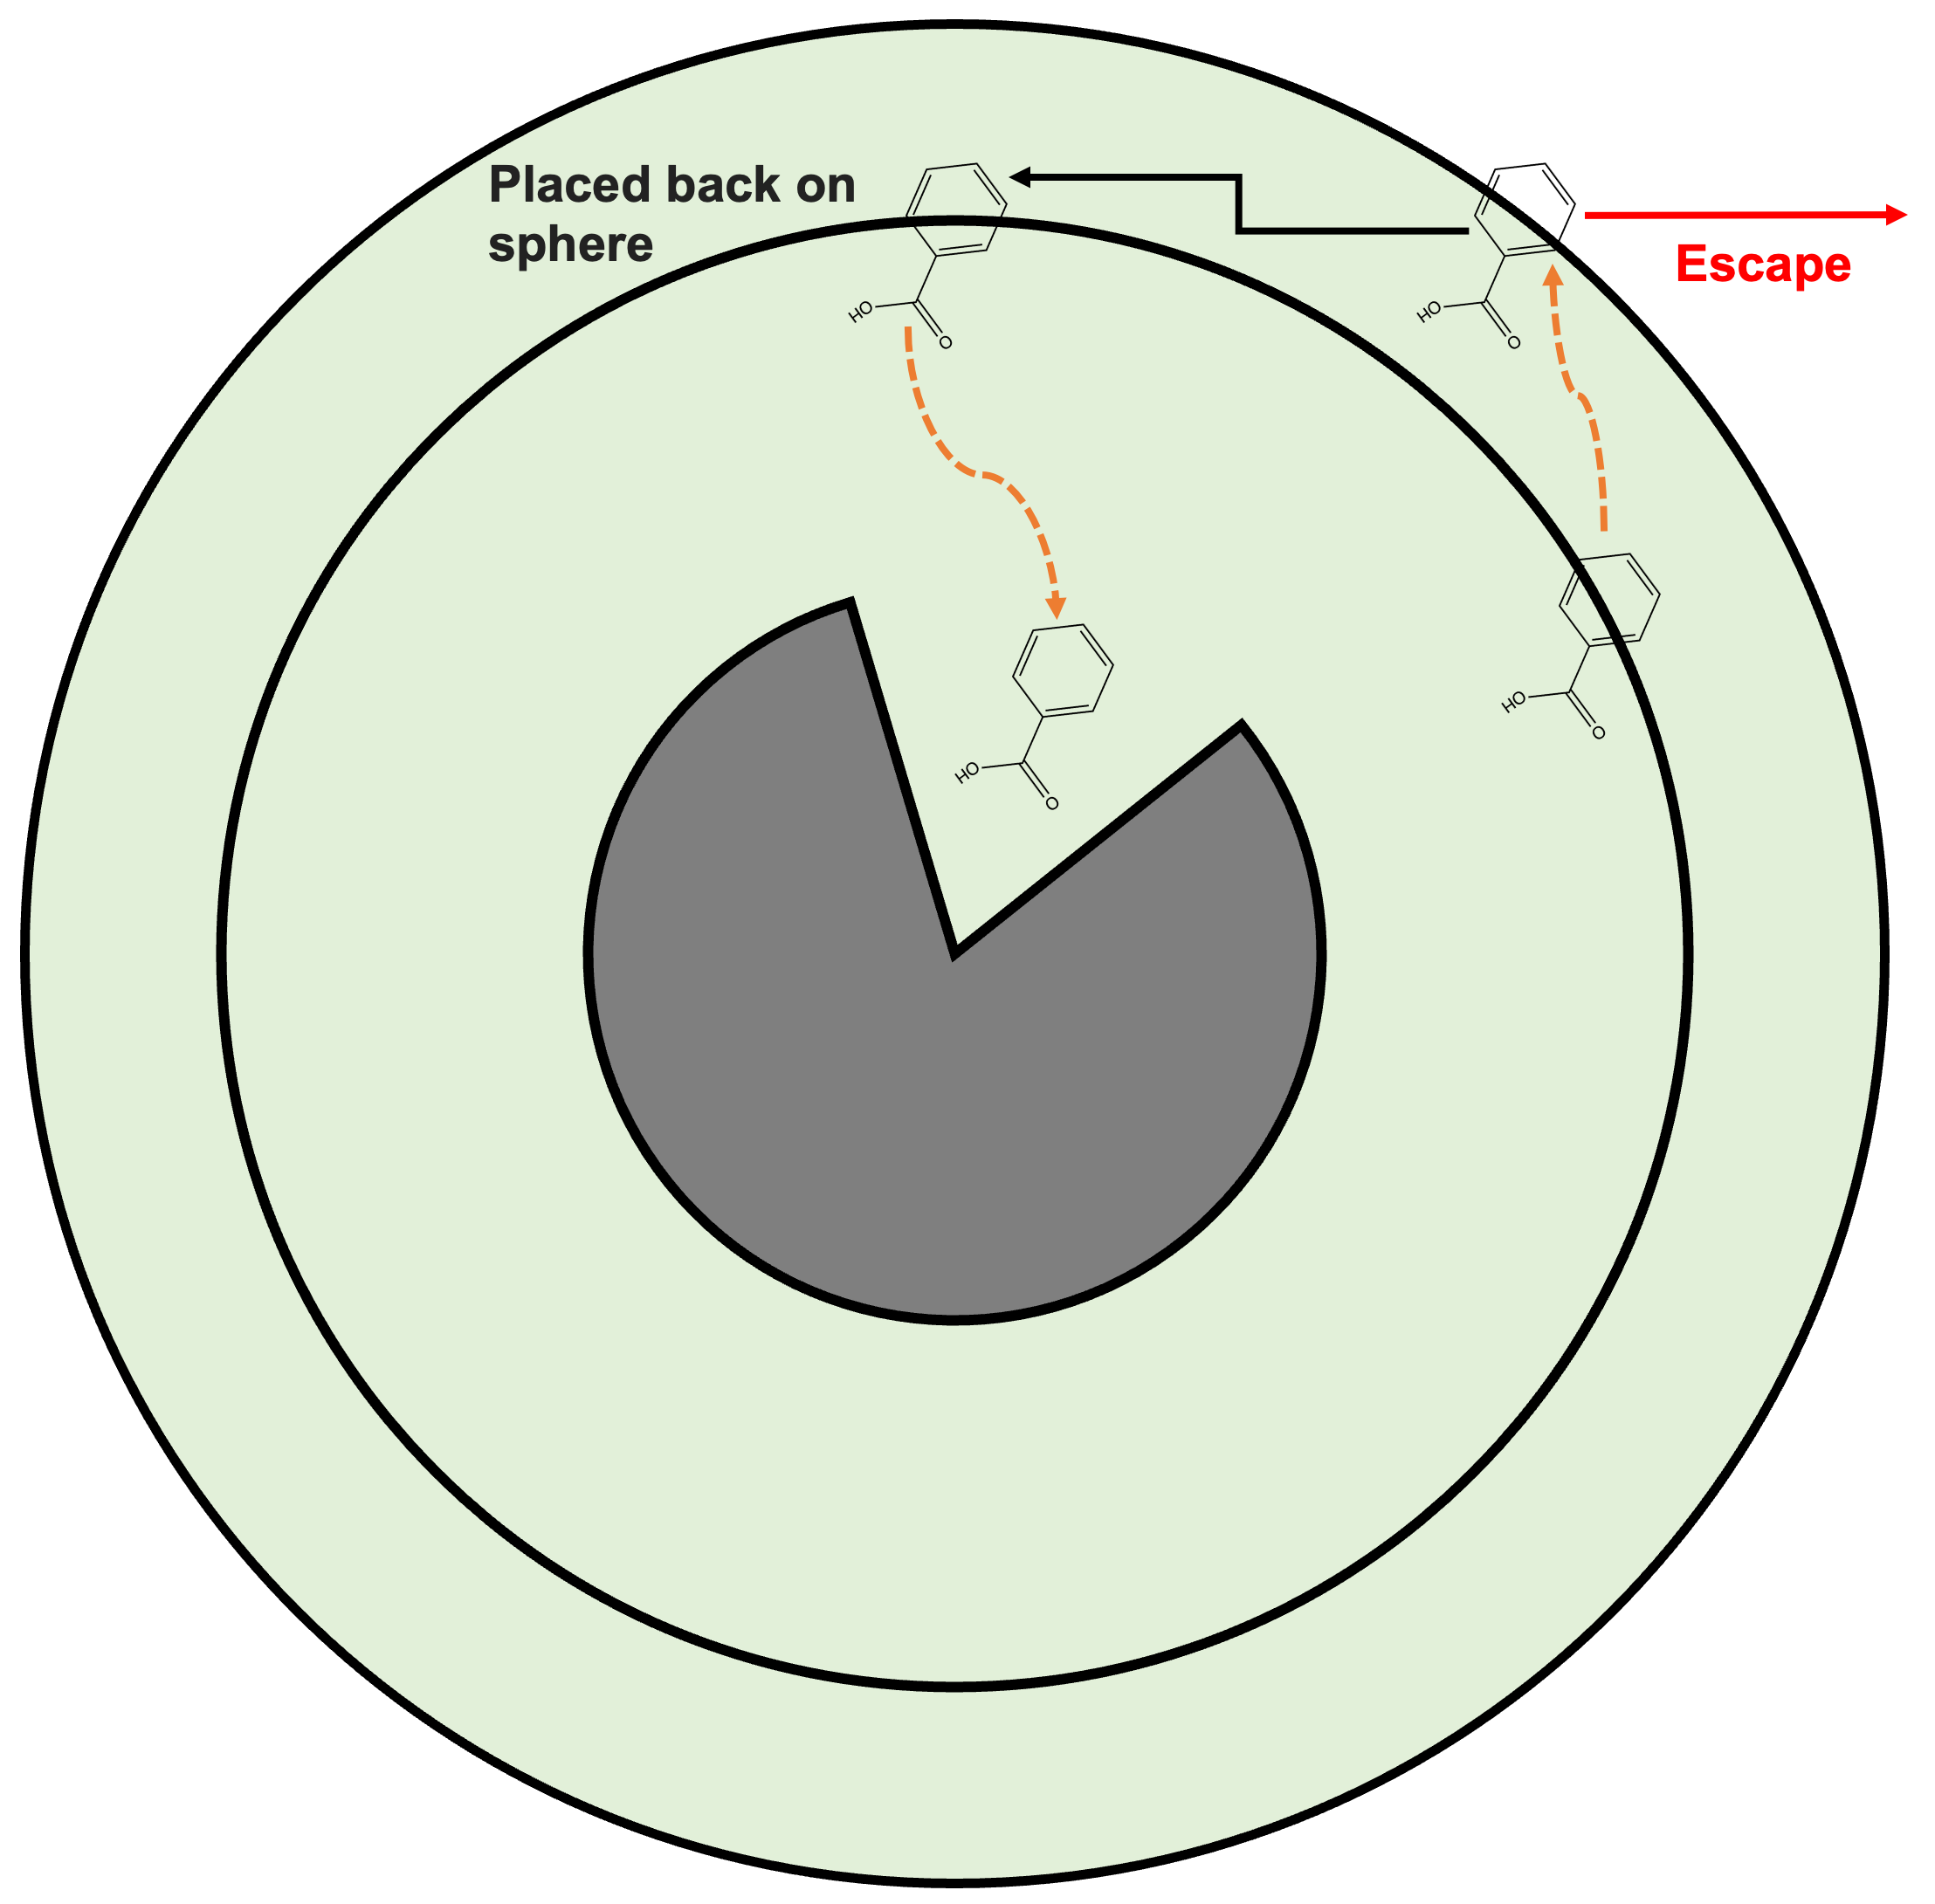
\includegraphics[scale=0.48]{images/figure1.png}
\caption{Computation of association rate using the Luty-McCammon-Zhou method}
\label{figure1}
\end{figure}

\noindent Given the simplifications and speedup of using BD simulations, it is possible to generate elongated trajectories of the ligand in the space around the receptor to estimate the association rate. Browndye2 uses the Luty-McCammon-Zhou algorithm (Figure \ref{figure1}) \cite{luty1992diffusive} (a variation of the earlier Northrup-Allison-McCammon algorithm \cite{northrup1984brownian}), which generates multiple trajectories, each of which ends either in an encounter with the receptor, or an escape. The ligand is started on a sphere surrounding the receptor and moves until it either reaches a final encounter with the receptor or reaches another sphere, larger and concentric with the first. If it reaches this second sphere, it either escapes, ending the trajectory, or it is placed back on the first sphere to continue the trajectory. The probability of the escape versus continuing from the inner sphere depends on several factors, such as the diameters of the spheres, the total charge on each system (ligand and the receptor), and the ionic strength of the solvent. Ultimately, the second-order association rate constant is computed from the proportion of encounters to escapes, and therefore a large number of trajectories are required to estimate that probability precisely. When used with SEEKR2, the encounter complex is defined as the ligand reaching the outermost milestone that encompasses the MD region. The milestoning calculations, with their parameters computed from the MD simulations, convert this initial rate constant into the final rate constant estimate, which accounts for the atomic details in the binding site, as described in section \ref{mmvt} and \ref{seekr_framework}. \par

\vspace{2mm}

\subsection{Markovian milestoning with Voronoi tessellations} \label{mmvt}
\vspace{2mm}

Milestoning is a phase-space splitting strategy for enhanced MD sampling. For a thorough understanding of the milestoning theory, readers are advised to refer to the key papers by Elber and coworkers \cite{vanden2008assumptions, bello2015exact, elber2020milestoning}. A series of mathematical equations are employed in the SEEKR2 milestoning methodology for calculating the mean first passage time (MFPT) and free energy related to binding for each milestone ($\Delta$G\textsubscript{i}). This tutorial recognizes the value of revisiting essential equations from our earlier works. Previous SEEKR2 publications employ the following mathematical representations \cite{jagger2020predicting, votapka2022seekr2, ojha2022selectivity, ojha2023qmrebind}. For the sake of comprehensiveness and to ensure this tutorial remains a self-contained resource, we have chosen to present these equations again. \par

\noindent Let us begin by segmenting the phase configuration of a bimolecular complex into \textit{N} distinct milestones. The transitions between milestones is described in the transition rate matrix, \textbf{Q}, of size \textit{N} $\times$ \textit{N}, which represents the fluxes across milestones, as shown in equation \ref{eqa}. The matrix \textbf{Q} consists of diagonal elements, \textit{q}\textsubscript{ii}, and off-diagonal elements, \textit{q}\textsubscript{ij}. 

\begin{equation}
\textbf{Q} = \begin{pmatrix}
q_{1,1} & q_{1,2} & \cdots & q_{1,N} \\
q_{2,1} & q_{2,2} & \cdots & q_{2,N} \\
\vdots  & \vdots  & \ddots & \vdots  \\
q_{N,1} & q_{N,2} & \cdots & q_{N,N}
\end{pmatrix}
\label{eqa}
\end{equation}


\noindent Given the number of transitions between milestones \textit{i} and \textit{j} as \textit{N}\textsubscript{ij}, with the \textit{i}\textsuperscript{th} milestone as the last milestone the trajectory has interacted with, and \textit{R}\textsubscript{i} represents the duration the trajectory has spent in the particular milestone, the expressions for \textit{q}\textsubscript{ii} and \textit{q}\textsubscript{ij} are given by equations \ref{eqb} and \ref{eqc} respectively.

\begin{equation}
q_{ii} = - \sum_{j \neq i} q_{ij}
\label{eqb}
\end{equation}

\begin{equation}
q_{ij} =
\begin{cases}
\frac{N_{ij}}{R_i} & \text{if $R_i \neq 0$} \\
0 & \text{if $R_i = 0$}
\end{cases}
\label{eqc}
\end{equation}

\noindent For a trajectory within the Voronoi cell, $V$\textsubscript{$\alpha$}, its position and velocity vectors are denoted as $x$\textsubscript{$\alpha$} and $v$\textsubscript{$\alpha$} respectively. The position and velocity of this trajectory at time, \textit{t} + $\Delta$\textit{t}, as estimated by the integrator algorithm (Langevin integrator, at most times), are given by $x\textsubscript{$\alpha$}^{*}$ and $v\textsubscript{$\alpha$}^{*}$. Equations \ref{eqd} and \ref{eqe} enforce reflective boundaries to ensure trajectories are confined to their respective Voronoi cells.

\begin{equation}
x_{\alpha}(t+\Delta t)=
\begin{cases}
{x_{\alpha}}^* & \text{if } {x_{\alpha}}^* \in V_{\alpha} \\
{x_{\alpha}}(t) & \text{otherwise}
\end{cases}
\label{eqd}
\end{equation}

\begin{equation}
v_{\alpha}(t+\Delta t)=
\begin{cases}
{v_{\alpha}}^* & \text{if } {x_{\alpha}}^* \in V_{\alpha} \\
-{v_{\alpha}}(t) & \text{otherwise}
\end{cases}
\label{eqe}
\end{equation}

\noindent The equilibrium probabilities of Voronoi cells $V$\textsubscript{$\alpha$} and $V$\textsubscript{$\beta$} are represented by $\pi$\textsubscript{$\alpha$} and $\pi$\textsubscript{$\beta$} respectively, with the total simulation time within these cells given by $T_{\alpha}$ and $T_{\beta}$. A dimension-consistent normalization factor, \textit{T}, is given by equation \ref{eqf}.

\begin{equation}
T = \left(\sum_{\alpha=1}^{n} \frac{{\pi_{\alpha}}}{{T_{\alpha}}}\right)^{-1}
\label{eqf}
\end{equation}

\noindent If $N_{ij}^{\alpha}$ denotes the number of collisions with the \textit{j}\textsuperscript{th} milestone after last visiting the \textit{i}\textsuperscript{th} milestone (in this context, both the \textit{i}\textsuperscript{th} and \textit{j}\textsuperscript{th} milestone are edges to anchor $\alpha$), the total transitions between the  i\textsuperscript{th} and j\textsuperscript{th} milestones, N\textsubscript{ij}, is given by equation \ref{eqg}, as formulated in the original Markovian milestoning with Voronoi tesselations (MMVT) theory. \cite{vanden2008assumptions}

\begin{equation}
N_{ij} = T \sum_{\alpha=1}^{n} \pi_{\alpha} \frac{N_{ij}^{\alpha}}{T_{\alpha}}
\label{eqg}
\end{equation}

\noindent Given \textit{R}\textsubscript{i}\textsuperscript{$\alpha$} represents the time a trajectory spends in Voronoi cell $V$\textsubscript{$\alpha$} after its last interaction with the \textit{i}\textsuperscript{th} milestone, the aggregate time post the last interaction with the \textit{i}\textsuperscript{th} milestone, \textit{R}\textsubscript{i}, is given by equation \ref{eqh}.

\begin{equation}
R_{i} = T \sum_{\alpha=1}^{n} \pi_{\alpha} \frac{R_{i}^{ \alpha}}{T_{\alpha}}
\label{eqh}
\end{equation}

\noindent To compute the stationary probabilities \textbf{$\pi$}, one must consider both $N_{\alpha,\beta}$ (number of collisions in Voronoi cell $V_{\alpha}$ that occur at its boundary shared with $V_{\beta}$) and $N_{\beta,\alpha}$ (number of collisions in $V_{\beta}$ at its shared boundary with $V_{\alpha}$), as given by equations \ref{eqi} and \ref{eqj}.

\begin{equation}
\sum_{\beta=1, \beta \neq \alpha}^{n} \pi_{\beta} \frac{N_{\beta, \alpha}} {T_{\beta}} = \sum_{\beta=1, \beta \neq \alpha}^{n} \pi_{\alpha} \frac{N_{\alpha, \beta}} {T_{\alpha}}
\label{eqi}
\end{equation}

\begin{equation}
\sum_{\alpha=1}^{n} \pi_{\alpha} = 1
\label{eqj}
\end{equation}

\noindent Consider $\overset{\wedge}{\textbf{Q}}$ as the matrix of size \textit{N}-1 by \textit{N}-1 extracted from the upper left portion of \textbf{Q}. The rationale behind selecting the upper left section of the matrix \textbf{Q} while omitting the last column and row is to establish a “sink state" required to compute a kinetic quantity. By excluding the final column and row from \textbf{Q}, we effectively designate the state denoted by that particular row and column as the sink state. The vector \textbf{1} represents a vector of ones, the mean free passage times from each milestone, \textbf{T}$^{N}$, can be determined by solving equation \ref{eqk}.

\begin{equation}
\overset{\wedge}{\textbf{Q}} \textbf{T}^{N} = - \textbf{1}
\label{eqk}
\end{equation}

\noindent The stationary probabilities of the milestones, \textbf{p}, are obtained by solving equation \ref{eql}.

\begin{equation}
\textbf{Q}\textbf{p}=\textbf{p}
\label{eql}
\end{equation}

\noindent The stationary probabilities for the \textit{i}\textsuperscript{th} milestone and the reference milestone are represented by {\textit{p\textsubscript{i}}} and {\textit{p\textsubscript{ref}}}, respectively. Using these parameters, the free energy landscape for the \textit{i}\textsuperscript{th} milestone, $\Delta$G\textsubscript{i}, is given by equation \ref{eqm}, where k\textsubscript{$\mathrm{B}$} stands for Boltzmann's constant and \text{T} designates the temperature. 

\begin{equation}
\Delta G_{i} = - k_{\mathrm{B}} \text{T} \ln\left(\frac{p_{i}}{p_{\mathrm{ref}}}\right)
\label{eqm}
\end{equation}

\subsection{The SEEKR2 workflow} \label{seekr_framework}

\vspace{2mm}

Let us consider the case of a model receptor-ligand complex to understand the steps involved in the SEEKR2 workflow. Initially, a structural (PDB) file containing the receptor protein and the ligand in an explicit solvent is provided as an input file (Figure \ref{figure2}a).

\begin{figure}[H]
\centering
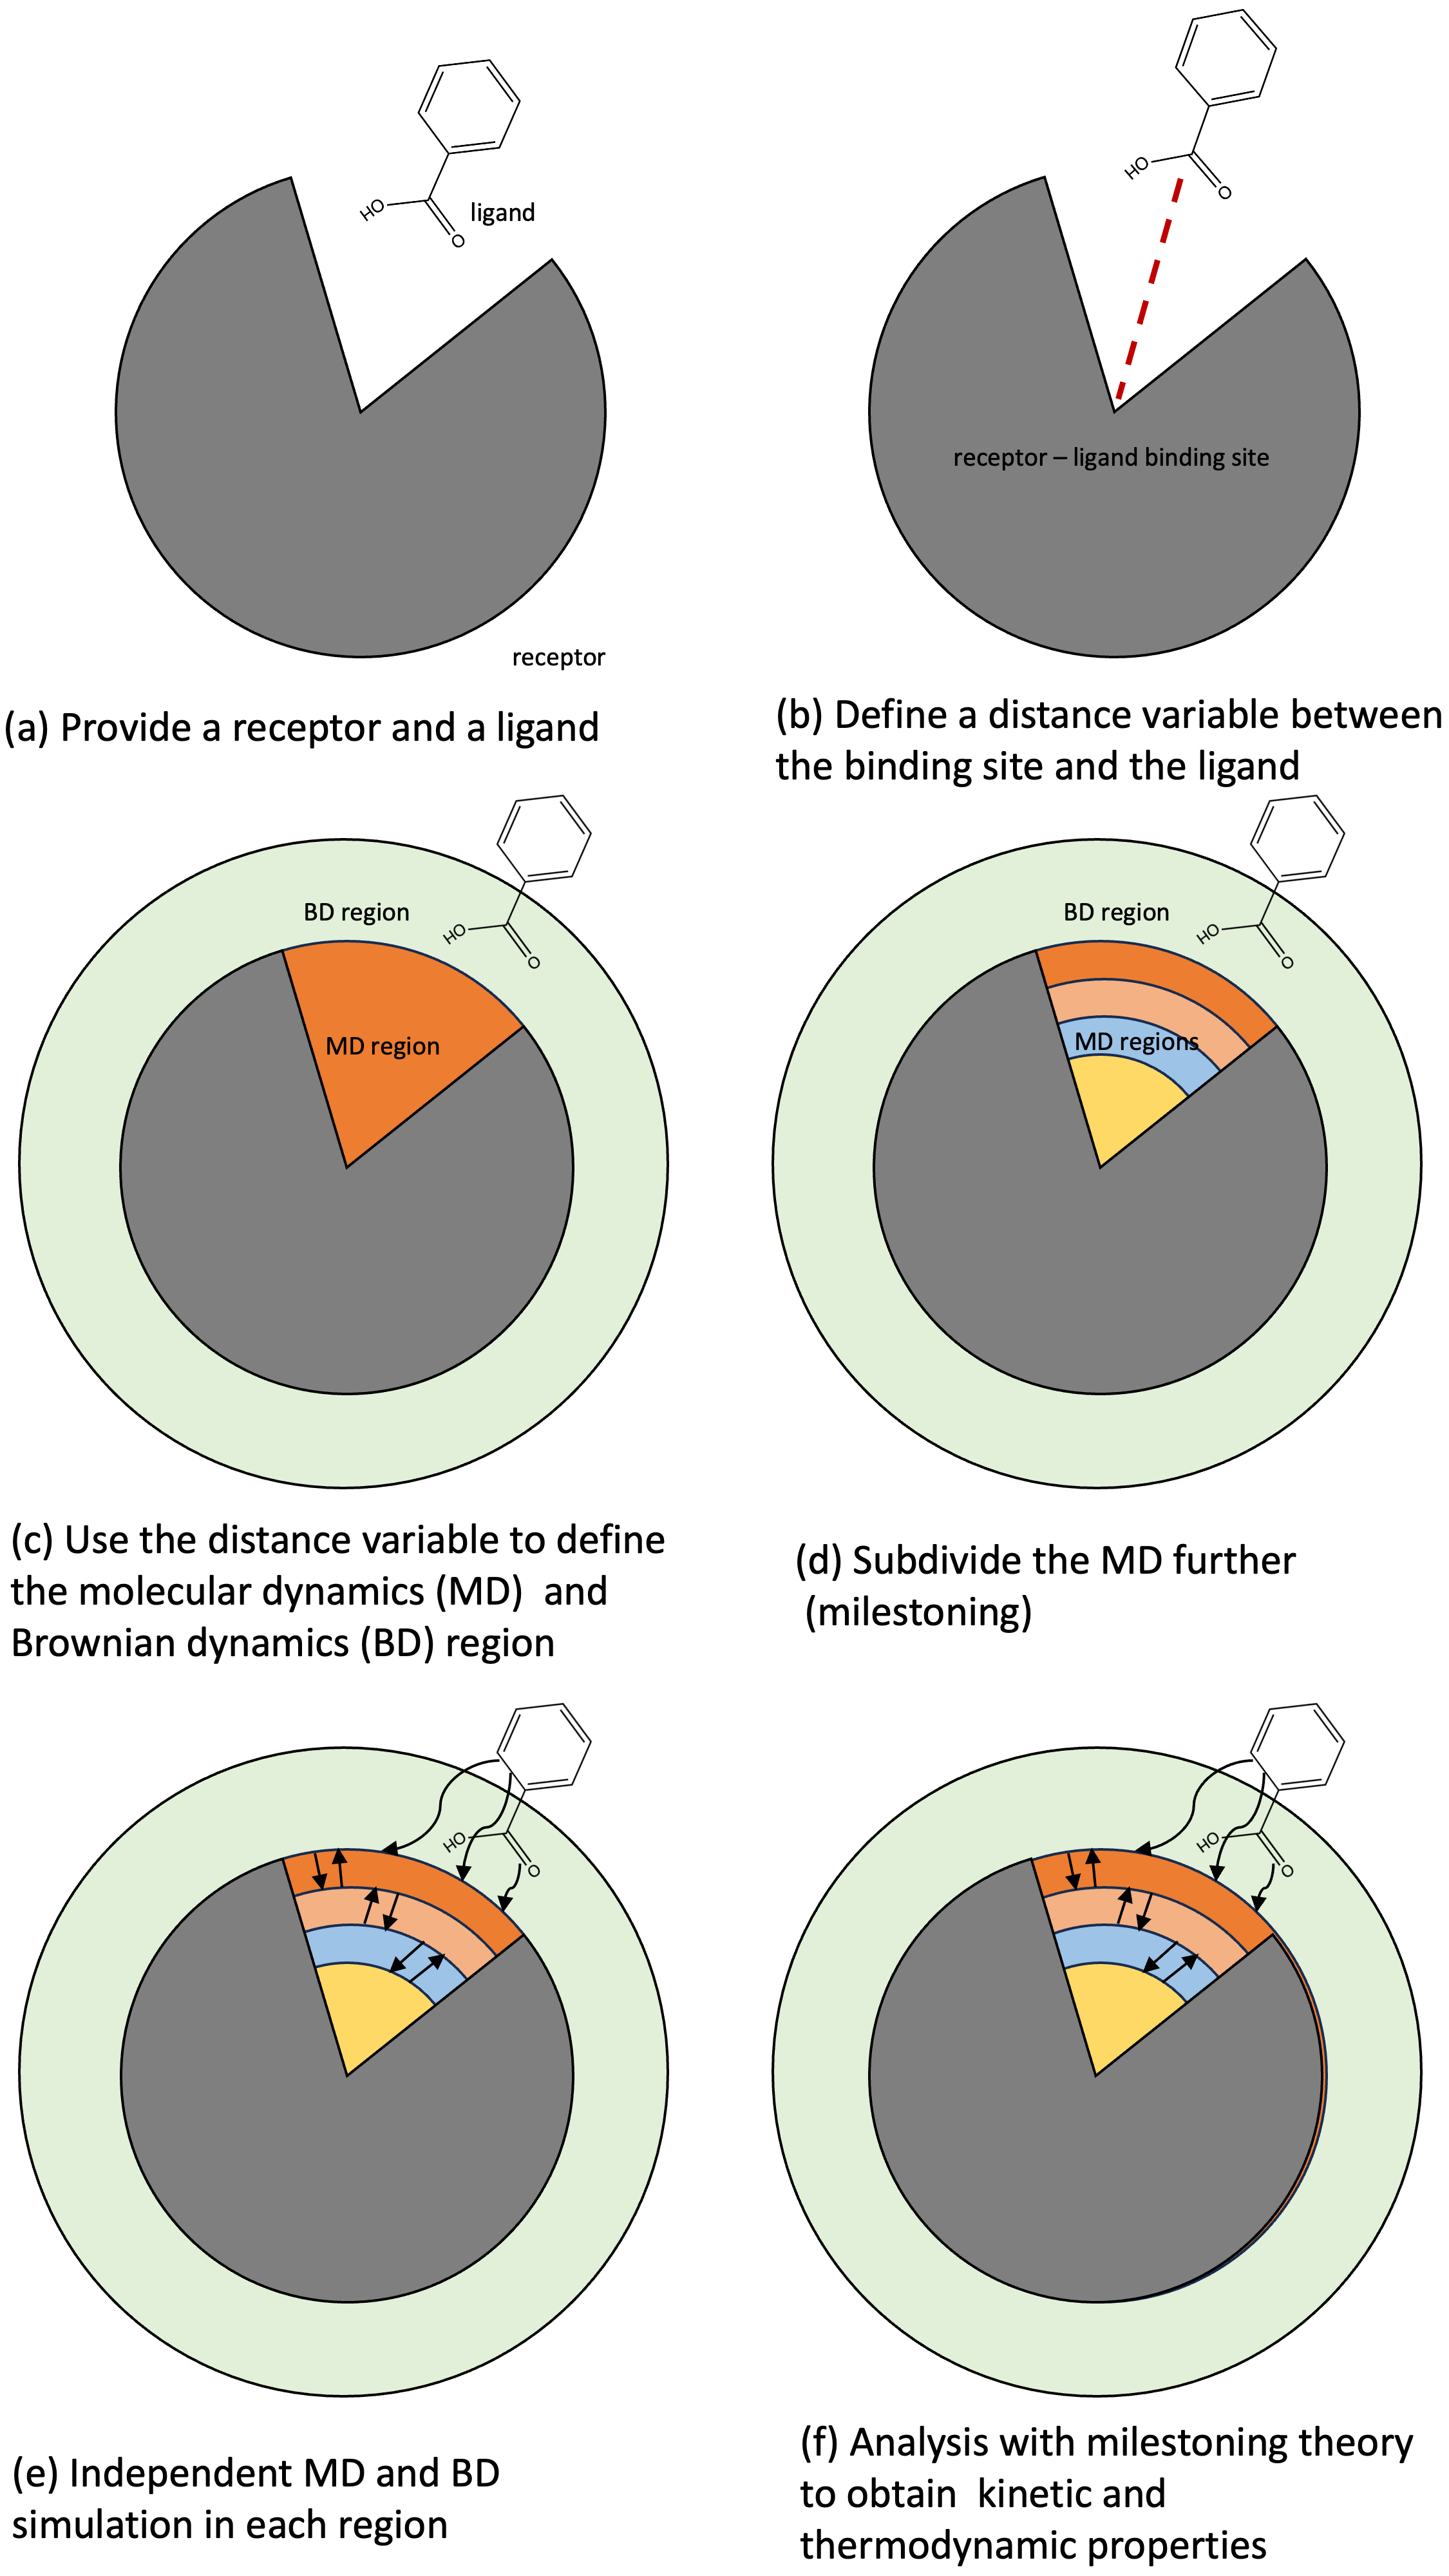
\includegraphics[scale=0.45]{images/figure2.png} 
\caption{Different stages of the SEEKR2 simulation framework}
\label{figure2}
\end{figure} 

\begin{figure}[H]
\centering
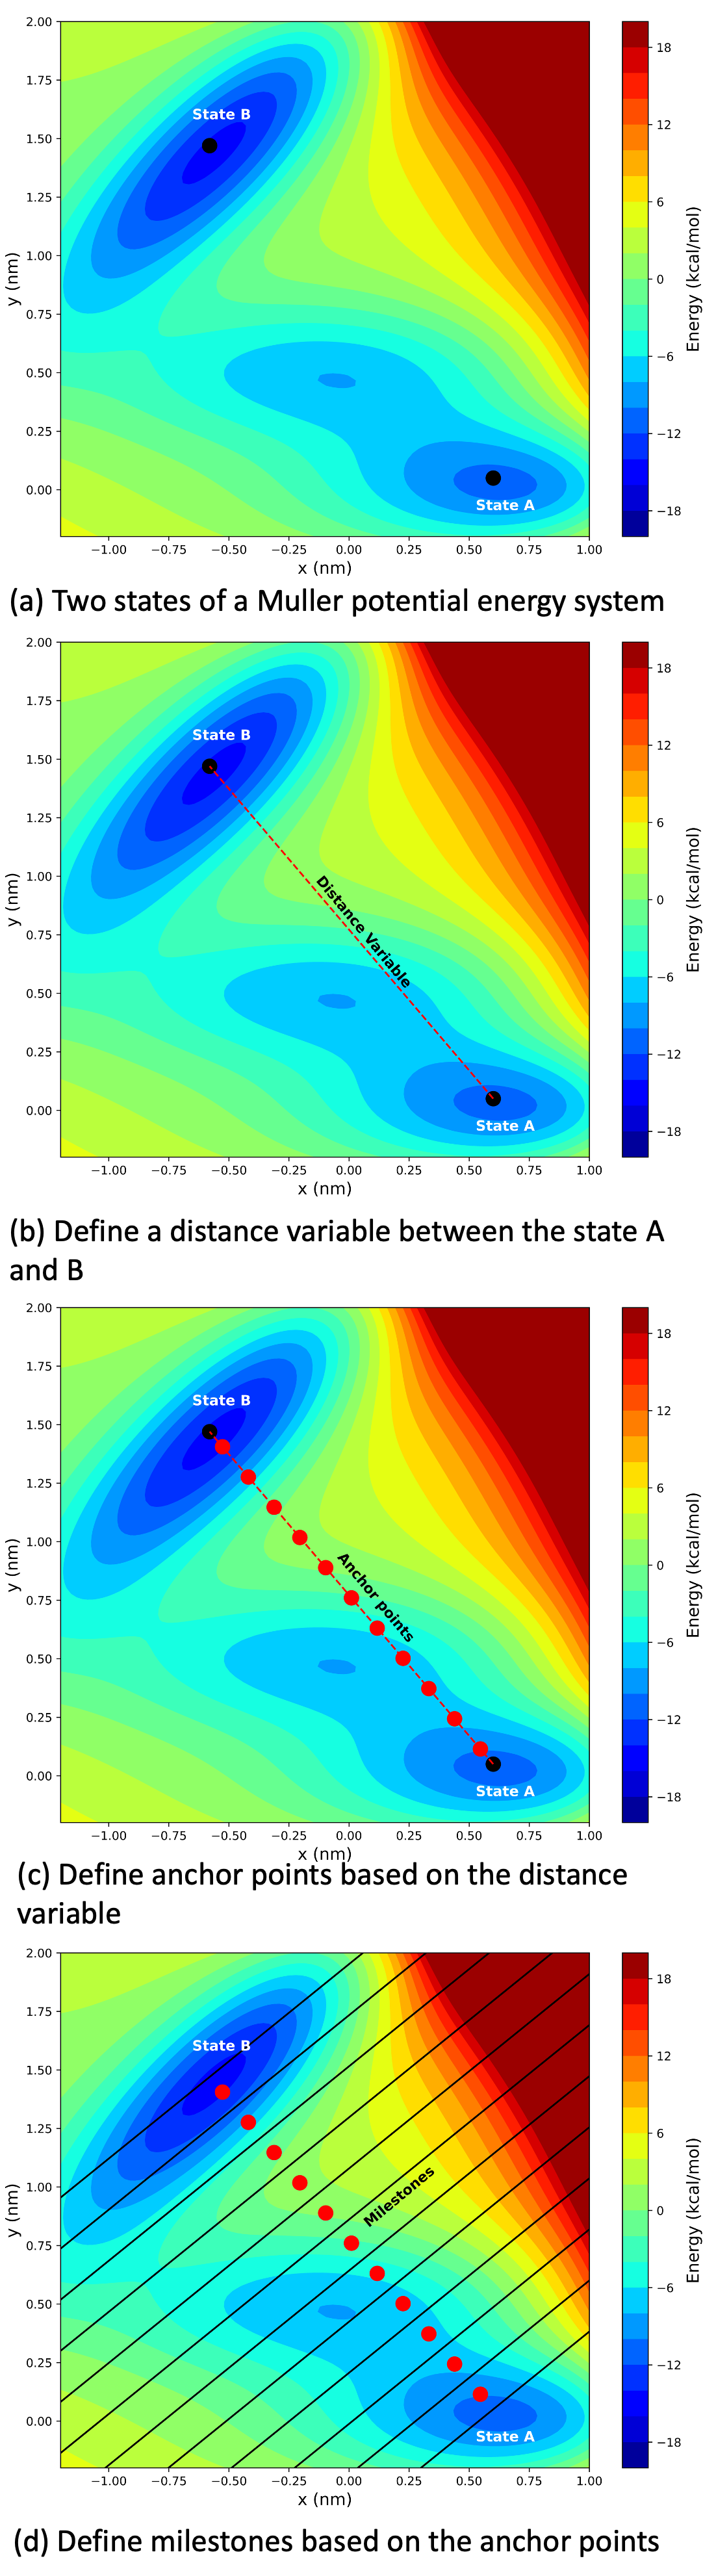
\includegraphics[scale=0.67]{images/figure3.png} 
\caption{A MMVT model of a simple Muller potential system within the SEEKR2 framework}
\label{figure3}
\end{figure} 

\noindent We then identify the ligand in the PDB file through its atom indices. Once the ligand and the receptor protein are identified, we define a collective variable (CV). In most cases, for receptor-ligand binding and unbinding processes, we choose the CV to be the distance between the center of mass (COM) of $\alpha$-carbon atoms at the binding site of the receptor and the COM of the heavy atoms of the ligand (Figure \ref{figure2}b). \par

\noindent Atomistic simulation details are required for receptor-ligand complexes when the ligand is close to the binding site, and conformational changes in the receptor are observed as the ligand slowly unbinds. In cases where the ligand is far from the receptor-ligand binding site, these two entities can be treated as point charges. Hence, BD is employed beyond a cut-off distance defined by the user.  Therefore, the phase space of the receptor-ligand complex is comprised of the MD region and the BD region (Figure \ref{figure2}c). We further subdivide the MD region into milestones based on a pre-defined CV. In one dimension, these milestones are concentric spheres with radii based on the increasing distance between the COM of the receptor-ligand binding site and the ligand (Figure \ref{figure2}d). \par

\noindent Independent MD and BD simulations are performed with reflective boundary conditions imposed within the MD Voronoi cells (Figure \ref{figure2}e). Once the simulation finishes, we can use milestoning theory to obtain the receptor-ligand unbinding rate (k\textsubscript{off}) and the addition of BD theory to obtain the receptor-ligand binding rate (k\textsubscript{on}) (Figure \ref{figure2}f). Thermodynamic parameters can then be obtained from the kinetic rates, k\textsubscript{on} and k\textsubscript{off}. \par 

\noindent To further understand the process of milestoning employed in the SEEKR2 framework, let us consider a system exhibiting a simple Muller potential, where an energy barrier exists between the two equilibrium states, A and B (Figure \ref{figure3}a). Let us define a CV as a distance variable that approximately describes the transition from state A to state B (Figure \ref{figure3}b). Anchor points are placed equidistant along the distance variable, constituting the points of a one-dimensional Voronoi tesselation (Figure \ref{figure3}c). Once the anchor points are defined, milestones are placed between the anchor points (Figure \ref{figure3}d). Independent and parallel MD simulations are run in the region defined by two successive milestones with reflective boundary conditions. \par

\section{SEEKR2 Installation}

\vspace{2mm}

\noindent Before proceeding with the SEEKR2 installation, we assume that the user has a working knowledge of Linux and has successfully installed the Anaconda or Miniconda distribution in the system. This tutorial also assumes the user possesses a computer with one or more graphical processing units (GPUs) capable of installing GPU-enabled software and running MD simulations on GPUs.

\subsection{Creating a new conda environment}
\vspace{2mm}
\begin{itemize} 

\item To verify the installation of conda in our system, we can run the following command in the terminal: 
\begin{tcolorbox}[colback=black!8!white, colframe=black!50!black, fontlower=\tiny, left=2pt, right=2pt, top=2pt, bottom=2pt] 
\texttt{which conda}
\end{tcolorbox}

If conda is properly installed, it will display the path to the conda executable.

\item We will create a dedicated conda environment for the SEEKR2 package. We execute the following command in the terminal to create a new environment named SEEKR2 with Python version 3.9:

\begin{tcolorbox}[colback=black!8!white, colframe=black!50!black, fontlower=\tiny, left=2pt, right=2pt, top=2pt, bottom=2pt] 
\texttt{conda create $-$$-$name SEEKR2 python=3.9}
\end{tcolorbox}

\item To use the SEEKR2 environment, we need to activate it by executing the following command in the terminal:

\begin{tcolorbox}[colback=black!8!white, colframe=black!50!black, fontlower=\tiny, left=2pt, right=2pt, top=2pt, bottom=2pt] 
\texttt{conda activate SEEKR2}
\end{tcolorbox}

\end{itemize}

\subsection{Installing SEEKR2 dependencies}
\vspace{2mm}

\begin{itemize}

\item We will ensure that the SEEKR2 conda environment is activated.

\begin{tcolorbox}[colback=black!8!white, colframe=black!50!black, fontlower=\tiny, left=2pt, right=2pt, top=2pt, bottom=2pt] 
\texttt{conda activate SEEKR2}
\end{tcolorbox}

\item To ensure that the Cython and git packages are installed, we execute the following commands in the terminal:

\begin{tcolorbox}[colback=black!8!white, colframe=black!50!black, fontlower=\tiny, left=2pt, right=2pt, top=2pt, bottom=2pt] 
\texttt{pip install $-$$-$upgrade cython}
\end{tcolorbox}

\begin{tcolorbox}[colback=black!8!white, colframe=black!50!black, fontlower=\tiny, left=2pt, right=2pt, top=2pt, bottom=2pt] 
\texttt{conda install git}
\end{tcolorbox}

\item For the proper execution of the tutorial scripts, we install the Ambertools and mdtraj packages via conda. 

\begin{tcolorbox}[colback=black!8!white, colframe=black!50!black, fontlower=\tiny, left=2pt, right=2pt, top=2pt, bottom=2pt] 
\texttt{conda install -c conda-forge ambertools}
\end{tcolorbox}

\begin{tcolorbox}[colback=black!8!white, colframe=black!50!black, fontlower=\tiny, left=2pt, right=2pt, top=2pt, bottom=2pt] 
\texttt{conda install -c conda-forge mdtraj}
\end{tcolorbox}

\item When installing SEEKR2 from source, we will also need to install the following additional packages (otherwise, not required for conda installation of SEEKR2):

\begin{tcolorbox}[colback=black!8!white, colframe=black!50!black, fontlower=\tiny, left=2pt, right=2pt, top=2pt, bottom=2pt] 
\texttt{conda install numpy}
\end{tcolorbox}

\begin{tcolorbox}[colback=black!8!white, colframe=black!50!black, fontlower=\tiny, left=2pt, right=2pt, top=2pt, bottom=2pt] 
\texttt{conda install scipy}
\end{tcolorbox}

\begin{tcolorbox}[colback=black!8!white, colframe=black!50!black, fontlower=\tiny, left=2pt, right=2pt, top=2pt, bottom=2pt] 
\texttt{conda install netcdf4}
\end{tcolorbox}

\begin{tcolorbox}[colback=black!8!white, colframe=black!50!black, fontlower=\tiny, left=2pt, right=2pt, top=2pt, bottom=2pt] 
\texttt{conda install mpi4py}
\end{tcolorbox}

\begin{tcolorbox}[colback=black!8!white, colframe=black!50!black, fontlower=\tiny, left=2pt, right=2pt, top=2pt, bottom=2pt] 
\texttt{conda install swig}
\end{tcolorbox}

\begin{tcolorbox}[colback=black!8!white, colframe=black!50!black, fontlower=\tiny, left=2pt, right=2pt, top=2pt, bottom=2pt] 
\texttt{conda install -c conda-forge doxygen}
\end{tcolorbox}

\noindent To install the ccmake package, sudo privileges are required (otherwise, not required for conda installation of SEEKR2). We execute the following command in the terminal:

\begin{tcolorbox}[colback=black!8!white, colframe=black!50!black, fontlower=\tiny, left=2pt, right=2pt, top=2pt, bottom=2pt] 
\texttt{sudo apt-get install cmake-curses-gui}
\end{tcolorbox}

\noindent To ensure the successful installation of ccmake, execute the following command:

\begin{tcolorbox}[colback=black!8!white, colframe=black!50!black, fontlower=\tiny, left=2pt, right=2pt, top=2pt, bottom=2pt] 
\texttt{which ccmake}
\end{tcolorbox}

\end{itemize}

\subsection{Installing Browndye} \label{browndye_installations}
\vspace{2mm}

\noindent Browndye2 (the latest version of the Browndye software) is compatible with various operating systems, including Linux, BSD, MacOS, and MS Windows. This tutorial will only provide instructions to install the Browndye package on Linux distributions. The recommended method for installing Browndye is to download the source code and compile it. Browndye relies on Ocaml and C++ compilers, with the C++17 version being the minimum requirement.

\begin{itemize}
\item We install the necessary package dependencies based on the Linux distribution:

\noindent For Ubuntu (20.04 and 22.04), we run the following command in the terminal:

\begin{tcolorbox}[colback=black!8!white, colframe=black!50!black, fontlower=\tiny, left=2pt, right=2pt, top=2pt, bottom=2pt] 
\texttt{apt-get install make gcc g++ ocaml \textbackslash \linebreak libexpat-dev liblapack-dev apbs}
\end{tcolorbox}

\noindent  For CentOS 7 distribution, we run the following commands to update the compilers and install the required packages:

\begin{tcolorbox}[colback=black!8!white, colframe=black!50!black, fontlower=\tiny, left=2pt, right=2pt, top=2pt, bottom=2pt] 
\texttt{yum install centos-release-scl epel-release} 
\end{tcolorbox}

\begin{tcolorbox}[colback=black!8!white, colframe=black!50!black, fontlower=\tiny, left=2pt, right=2pt, top=2pt, bottom=2pt] 
\texttt{yum install devtoolset-9 ocaml expat-devel \textbackslash \linebreak lapack-devel apbs}
\end{tcolorbox}

\begin{tcolorbox}[colback=black!8!white, colframe=black!50!black, fontlower=\tiny, left=2pt, right=2pt, top=2pt, bottom=2pt] 
\texttt{scl enable devtoolset-9 bash} 
\end{tcolorbox}


\item We will download the Browndye2 source code from \browndyelink. We recommend the user, though not required, to install the software in the home directory. We then extract the downloaded source code archive and install BrownDye2 by executing the following commands:

\begin{tcolorbox}[colback=black!8!white, colframe=black!50!black, fontlower=\tiny, left=2pt, right=2pt, top=2pt, bottom=2pt] 
\texttt{wget \browndyelink} 
\end{tcolorbox}

\begin{tcolorbox}[colback=black!8!white, colframe=black!50!black, fontlower=\tiny, left=2pt, right=2pt, top=2pt, bottom=2pt] 
\texttt{tar xvfz browndye2.tar.gz} 
\end{tcolorbox}

\begin{tcolorbox}[colback=black!8!white, colframe=black!50!black, fontlower=\tiny, left=2pt, right=2pt, top=2pt, bottom=2pt] 
\texttt{cd browndye2} 
\end{tcolorbox}

\begin{tcolorbox}[colback=black!8!white, colframe=black!50!black, fontlower=\tiny, left=2pt, right=2pt, top=2pt, bottom=2pt] 
\texttt{make -j 4 all} 
\end{tcolorbox}

\item Once we have finished unpacking the files, it is important to ensure that we include the installation location of the Browndye2 software in the system's PATH variable. This will allow us to run the software from any directory without specifying the full path each time. If the software has been installed in the home directory, we can add the path by using the following command:

\begin{tcolorbox}[colback=black!8!white, colframe=black!50!black, fontlower=\tiny, left=2pt, right=2pt, top=2pt, bottom=2pt] 
\texttt{export PATH=/home/USERNAME/browndye2/bin:\textbackslash \linebreak $\$$$\{$PATH$\}$} 
\end{tcolorbox} 

\item To remove the downloaded file that is no longer necessary, move to the folder where Browndye2 is installed and execute the following command:
\begin{tcolorbox}[colback=black!8!white, colframe=black!50!black, fontlower=\tiny, left=2pt, right=2pt, top=2pt, bottom=2pt] 
\texttt{rm browndye2.tar.gz } 
\end{tcolorbox}

\end{itemize}

\noindent Once the compilation process is complete, Browndye2 will be installed and ready to use on the Linux distribution.


\subsection{Conda installation of SEEKR2}
\vspace{2mm}

\subsubsection{Installing SEEKR2-OpenMM plugin}
\vspace{2mm}

\begin{itemize}

\item If not already activated, we first activate the SEEKR2 conda environment. 

\begin{tcolorbox}[colback=black!8!white, colframe=black!50!black, fontlower=\tiny, left=2pt, right=2pt, top=2pt, bottom=2pt] 
\texttt{conda activate SEEKR2}
\end{tcolorbox}

\item We will install the SEEKR2 plugin, which installs the OpenMM MD engine (version 7.7) and the CUDA Toolkit version 10.2 (compatible with SEEKR2), along with installing other dependencies.

\begin{tcolorbox}[colback=black!8!white, colframe=black!50!black, fontlower=\tiny, left=2pt, right=2pt, top=2pt, bottom=2pt] 
\texttt{conda install -c conda-forge \textbackslash \linebreak seekr2$\_$openmm$\_$plugin}
\end{tcolorbox}

\item To test the successful installation of SEEKR2, open a Python terminal and enter the following command: 
\begin{tcolorbox}[colback=black!8!white, colframe=black!50!black, fontlower=\tiny, left=2pt, right=2pt, top=2pt, bottom=2pt] 
\texttt{python} \\
\texttt{$>$$>$$>$ import seekr2plugin}
\end{tcolorbox}

\end{itemize}

\subsubsection{Installing SEEKR2} \label{seekrinstall}
\vspace{2mm}

\noindent
\begin{itemize}

\item If not already activated, we first activate the SEEKR2 conda environment. 

\begin{tcolorbox}[colback=black!8!white, colframe=black!50!black, fontlower=\tiny, left=2pt, right=2pt, top=2pt, bottom=2pt] 
\texttt{conda activate SEEKR2}
\end{tcolorbox}

\item It is recommended, though not required, to install the SEEKR2 program in the home directory. So, we navigate to the home directory. 

\begin{tcolorbox}[colback=black!8!white, colframe=black!50!black, fontlower=\tiny, left=2pt, right=2pt, top=2pt, bottom=2pt] 
\texttt{cd $\sim$}
\end{tcolorbox}

\item We will clone the SEEKR2 Python API repository by running the following command in the terminal:

\begin{tcolorbox}[colback=black!8!white, colframe=black!50!black, fontlower=\tiny, left=2pt, right=2pt, top=2pt, bottom=2pt] 
\texttt{git clone \seekrgithublink}
\end{tcolorbox}

\item We then proceed with the installation of SEEKR2 Python API in the cloned \textit{seekr2} directory:

\begin{tcolorbox}[colback=black!8!white, colframe=black!50!black, fontlower=\tiny, left=2pt, right=2pt, top=2pt, bottom=2pt] 
\texttt{cd seekr2} 
\end{tcolorbox}

\begin{tcolorbox}[colback=black!8!white, colframe=black!50!black, fontlower=\tiny, left=2pt, right=2pt, top=2pt, bottom=2pt] 
\texttt{python -m pip install .}
\end{tcolorbox}

\item Once the installation is complete, it is recommended to run tests to ensure the proper functioning of SEEKR2. From within the \textit{seekr2} directory, we execute the following command:

\begin{tcolorbox}[colback=black!8!white, colframe=black!50!black, fontlower=\tiny, left=2pt, right=2pt, top=2pt, bottom=2pt] 
\texttt{pytest}
\end{tcolorbox}

\end{itemize}
\noindent Running the tests may generate one or two failures depending on the availability of NAMD and Browndye2 software, which can safely be ignored if these programs are not required for your specific use case. SEEKR2 is now successfully installed on our system, and we can begin utilizing its features and functionalities.

\subsubsection{Installing Seekrtools}
\vspace{2mm}

\noindent Seekrtools is a suite of software utilities designed to work with SEEKR2 to streamline the preparation process and execution of multiscale milestoning simulations. For more comprehensive instructions and tutorials, please refer to the official documentation at \seekrtoolslink. Ensuring that SEEKR2 and OpenMM packages are installed before installing Seekrtools is crucial, as most programs within Seekrtools rely on these packages. \par

\begin{itemize}

\item If not already activated, we first activate the SEEKR2 conda environment. 

\begin{tcolorbox}[colback=black!8!white, colframe=black!50!black, fontlower=\tiny, left=2pt, right=2pt, top=2pt, bottom=2pt] 
\texttt{conda activate SEEKR2}
\end{tcolorbox}

\item It is recommended, though not required, to install the seekrtools program in the home directory. So, we navigate to the home directory. 

\begin{tcolorbox}[colback=black!8!white, colframe=black!50!black, fontlower=\tiny, left=2pt, right=2pt, top=2pt, bottom=2pt] 
\texttt{cd $\sim$}
\end{tcolorbox}

\item We will clone the seekrtools Python API repository by running the following command in the terminal:

\begin{tcolorbox}[colback=black!8!white, colframe=black!50!black, fontlower=\tiny, left=2pt, right=2pt, top=2pt, bottom=2pt] 
\texttt{git clone \seekrtoolsgithublink}
\end{tcolorbox}

\item We then proceed with the installation of seekrtools Python API in the cloned \textit{seekrtools} directory:

\begin{tcolorbox}[colback=black!8!white, colframe=black!50!black, fontlower=\tiny, left=2pt, right=2pt, top=2pt, bottom=2pt] 
\texttt{cd seekrtools} 
\end{tcolorbox}

\begin{tcolorbox}[colback=black!8!white, colframe=black!50!black, fontlower=\tiny, left=2pt, right=2pt, top=2pt, bottom=2pt] 
\texttt{python -m pip install .}
\end{tcolorbox}

\item Once the installation is complete, it is recommended to run tests to ensure the proper functioning of seekrtools. From within the \textit{seekrtools} directory, we execute the following command:

\begin{tcolorbox}[colback=black!8!white, colframe=black!50!black, fontlower=\tiny, left=2pt, right=2pt, top=2pt, bottom=2pt] 
\texttt{pytest}
\end{tcolorbox}

\end{itemize}

\subsection{Installing SEEKR2 from source}
\vspace{2mm}

\subsubsection{Installing OpenMM from source} \label{openmm_installation_source}
\vspace{2mm}

\noindent Sometimes, a SEEKR2 installation from conda-forge will not be possible or desirable. In those cases, one will need to perform the more arduous and difficult process of installing OpenMM and the SEEKR2 OpenMM Plugin from source. Before installing the OpenMM package, it is essential to install CUDA. Please follow NVIDIA's CUDA toolkit installation manual instructions and refer to the documentation at \cudatutoriallink. Carefully read and follow the steps outlined in the guide to ensure a successful CUDA installation. Once CUDA is installed, we can proceed with installing the OpenMM package. \par

\begin{itemize}

\item If not already activated, we first activate the SEEKR2 conda environment. 

\begin{tcolorbox}[colback=black!8!white, colframe=black!50!black, fontlower=\tiny, left=2pt, right=2pt, top=2pt, bottom=2pt] 
\texttt{conda activate SEEKR2}
\end{tcolorbox}

\item It is recommended, though not required, to install the OpenMM repository in the home directory. So, we navigate to the home directory. 

\begin{tcolorbox}[colback=black!8!white, colframe=black!50!black, fontlower=\tiny, left=2pt, right=2pt, top=2pt, bottom=2pt] 
\texttt{cd $\sim$}
\end{tcolorbox}

\item To clone the OpenMM repository:

\begin{tcolorbox}[colback=black!8!white, colframe=black!50!black, fontlower=\tiny, left=2pt, right=2pt, top=2pt, bottom=2pt] 
\texttt{git clone \openmmgithublink} 
\end{tcolorbox}

\item We then navigate to the \textit{openmm} directory:

\begin{tcolorbox}[colback=black!8!white, colframe=black!50!black, fontlower=\tiny, left=2pt, right=2pt, top=2pt, bottom=2pt] 
\texttt{cd openmm} 
\end{tcolorbox}

\item Create a \textit{build} directory:

\begin{tcolorbox}[colback=black!8!white, colframe=black!50!black, fontlower=\tiny, left=2pt, right=2pt, top=2pt, bottom=2pt] 
\texttt{mkdir build} 
\end{tcolorbox}

\item To navigate to the build directory:

\begin{tcolorbox}[colback=black!8!white, colframe=black!50!black, fontlower=\tiny, left=2pt, right=2pt, top=2pt, bottom=2pt] 
\texttt{cd build} 
\end{tcolorbox}

\item To configure the build using ccmake:

\begin{tcolorbox}[colback=black!8!white, colframe=black!50!black, fontlower=\tiny, left=2pt, right=2pt, top=2pt, bottom=2pt] 
\texttt{ccmake ..} 
\end{tcolorbox}

\noindent The above command opens the ccmake GUI. Press 'c' to configure and 't' to toggle advanced mode. We now modify the necessary variables in the ccmake GUI. We will set CMAKE$\_$INSTALL$\_$PREFIX to a local directory where we want to install the OpenMM engine (e.g., \textit{/home/USERNAME/bin/openmm}). If the directory does not exist, we will create it. Alternatively, we can leave this variable the default if we have sudo privileges and want to install OpenMM globally. We will then review and modify any other variables if needed. After modifying the variables, we press 'c' to configure. If any issues arise, ccmake will notify us. Once the configuration is successful, we press 'g' to generate the build files. The ccmake GUI will then close automatically.

\item To install OpenMM, execute the following commands in the \textit{build} directory:

\begin{tcolorbox}[colback=black!8!white, colframe=black!50!black, fontlower=\tiny, left=2pt, right=2pt, top=2pt, bottom=2pt] 
\texttt{make} 
\end{tcolorbox}

\begin{tcolorbox}[colback=black!8!white, colframe=black!50!black, fontlower=\tiny, left=2pt, right=2pt, top=2pt, bottom=2pt] 
\texttt{make install} 
\end{tcolorbox}

\begin{tcolorbox}[colback=black!8!white, colframe=black!50!black, fontlower=\tiny, left=2pt, right=2pt, top=2pt, bottom=2pt] 
\texttt{make PythonInstall} 
\end{tcolorbox}

\item To test the successful installation of OpenMM:

\begin{tcolorbox}[colback=black!8!white, colframe=black!50!black, fontlower=\tiny, left=2pt, right=2pt, top=2pt, bottom=2pt] 
\texttt{python -m openmm.testInstallation} 
\end{tcolorbox}

\noindent The above command will run a series of tests to ensure OpenMM is installed correctly on our system. 

\end{itemize}

\noindent We have now installed OpenMM and its plugins from the source on our local machine.

\subsubsection{Installing SEEKR2-OpenMM plugin from source}
\vspace{2mm}

\noindent Once the OpenMM engine is installed, we will install the SEEKR2 plugin on top of the installed version of OpenMM. It is recommended, though not required, to install the plugin in the home directory. 

\begin{itemize}

\item If not already activated, we first activate the SEEKR2 conda environment. 

\begin{tcolorbox}[colback=black!8!white, colframe=black!50!black, fontlower=\tiny, left=2pt, right=2pt, top=2pt, bottom=2pt]  
\texttt{conda activate SEEKR2}
\end{tcolorbox}

\item It is recommended, though not required, to install the SEEKR2 plugin in the home directory. So, we navigate to the home directory. 

\begin{tcolorbox}[colback=black!8!white, colframe=black!50!black, fontlower=\tiny, left=2pt, right=2pt, top=2pt, bottom=2pt] 
\texttt{cd $\sim$}
\end{tcolorbox}

\item To clone the SEEKR2-OpenMM plugin repository:

\begin{tcolorbox}[colback=black!8!white, colframe=black!50!black, fontlower=\tiny, left=2pt, right=2pt, top=2pt, bottom=2pt]  
\texttt{git clone \seekropenmmpluginlink}
\end{tcolorbox}

\item We then navigate to into the \textit{seekr2$\_$openmm$\_$plugin} directory:

\begin{tcolorbox}[colback=black!8!white, colframe=black!50!black, fontlower=\tiny, left=2pt, right=2pt, top=2pt, bottom=2pt]  
\texttt{cd seekr2$\_$openmm$\_$plugin/seekr2plugin}
\end{tcolorbox}

\item Create a \textit{build} directory:

\begin{tcolorbox}[colback=black!8!white, colframe=black!50!black, fontlower=\tiny, left=2pt, right=2pt, top=2pt, bottom=2pt] 
\texttt{mkdir build} 
\end{tcolorbox}

\item To navigate to the build directory:

\begin{tcolorbox}[colback=black!8!white, colframe=black!50!black, fontlower=\tiny, left=2pt, right=2pt, top=2pt, bottom=2pt] 
\texttt{cd build} 
\end{tcolorbox}

\item To configure the build using ccmake:

\begin{tcolorbox}[colback=black!8!white, colframe=black!50!black, fontlower=\tiny, left=2pt, right=2pt, top=2pt, bottom=2pt] 
\texttt{ccmake ..} 
\end{tcolorbox}

\noindent The above command opens the ccmake GUI. Press 'c' to configure. We now modify the necessary variables in the ccmake GUI. We will set CMAKE$\_$INSTALL$\_$PREFIX to the directory similar to the CMAKE$\_$INSTALL$\_$PREFIX as set during the OpenMM installation (e.g., \textit{/home/USERNAME/bin/openmm}). We will also set the OPENMM$\_$DIR to the directory similar to the CMAKE$\_$INSTALL$\_$PREFIX as set during the installation of OpenMM engine (e.g., \textit{/home/USERNAME/bin/openmm}). We will set the SEEKR2$\_$BUILD$\_$OPENCL$\_$LIB to OFF. After modifying the variables, we press 'c' to configure. If any issues arise, ccmake will notify us. Once the configuration is successful, we then press 'g' to generate the build files. The ccmake GUI will then close automatically.

\item To install the SEEKR2 plugin, we execute the following commands in the \textit{build} directory:

\begin{tcolorbox}[colback=black!8!white, colframe=black!50!black, fontlower=\tiny, left=2pt, right=2pt, top=2pt, bottom=2pt] 
\texttt{make} 
\end{tcolorbox}

\begin{tcolorbox}[colback=black!8!white, colframe=black!50!black, fontlower=\tiny, left=2pt, right=2pt, top=2pt, bottom=2pt] 
\texttt{make install} 
\end{tcolorbox}

\begin{tcolorbox}[colback=black!8!white, colframe=black!50!black, fontlower=\tiny, left=2pt, right=2pt, top=2pt, bottom=2pt] 
\texttt{make PythonInstall} 
\end{tcolorbox} 

\item To ensure proper installation of the SEEKR2 plugin, we execute the following command in the terminal:

\begin{tcolorbox}[colback=black!8!white, colframe=black!50!black, fontlower=\tiny, left=2pt, right=2pt, top=2pt, bottom=2pt] 
\texttt{make test} 
\end{tcolorbox} 

\end{itemize}

\subsubsection{Installing SEEKR2}
\vspace{2mm}

Please refer to section \ref{seekrinstall} for detailed instructions to install SEEKR2. However, for the sake of completion, we execute the following commands to install SEEKR2.  \par 

\begin{tcolorbox}[colback=black!8!white, colframe=black!50!black, fontlower=\tiny, left=2pt, right=2pt, top=2pt, bottom=2pt] 
\texttt{conda activate SEEKR2} \\
\texttt{$\#$ Activate SEEKR2 environment, if not activated} 
\end{tcolorbox}

\begin{tcolorbox}[colback=black!8!white, colframe=black!50!black, fontlower=\tiny, left=2pt, right=2pt, top=2pt, bottom=2pt] 
\texttt{cd $\sim$} \\
\texttt{$\#$ Navigate to home directory (recommended)} 
\end{tcolorbox}

\begin{tcolorbox}[colback=black!8!white, colframe=black!50!black, fontlower=\tiny, left=2pt, right=2pt, top=2pt, bottom=2pt] 
\texttt{git clone \seekrgithublink} \texttt{ \linebreak $\#$ Clone the SEEKR2 repository}
\end{tcolorbox}

\begin{tcolorbox}[colback=black!8!white, colframe=black!50!black, fontlower=\tiny, left=2pt, right=2pt, top=2pt, bottom=2pt] 
\texttt{cd seekr2} \\
\texttt{$\#$ Navigate to the \textit{seekr2} directory} 
\end{tcolorbox}

\begin{tcolorbox}[colback=black!8!white, colframe=black!50!black, fontlower=\tiny, left=2pt, right=2pt, top=2pt, bottom=2pt] 
\texttt{python -m pip install .} \\
\texttt{$\#$ Install SEEKR2}
\end{tcolorbox}

\begin{tcolorbox}[colback=black!8!white, colframe=black!50!black, fontlower=\tiny, left=2pt, right=2pt, top=2pt, bottom=2pt] 
\texttt{pytest} \\
\texttt{ $\#$ Run tests to check successful installation}
\end{tcolorbox}


\subsubsection{Installing Seekrtools}
\vspace{2mm}

\noindent Seekrtools is a suite of software utilities designed to work with SEEKR2 applications, primarily SEEKR2, to streamline the preparation process and execution of multiscale milestoning simulations. For more comprehensive instructions and tutorials, please refer to the official documentation at \seekrtoolslink. Ensuring that SEEKR2 and OpenMM packages are installed before installing Seekrtools is crucial, as most programs within Seekrtools rely on these packages. \par

\begin{itemize}

\item If not already activated, we first activate the SEEKR2 conda environment. 

\begin{tcolorbox}[colback=black!8!white, colframe=black!50!black, fontlower=\tiny, left=2pt, right=2pt, top=2pt, bottom=2pt] 
\texttt{conda activate SEEKR2}
\end{tcolorbox}

\item It is recommended, though not required, to install the seekrtools program in the home directory. So, we navigate to the home directory. 

\begin{tcolorbox}[colback=black!8!white, colframe=black!50!black, fontlower=\tiny, left=2pt, right=2pt, top=2pt, bottom=2pt] 
\texttt{cd $\sim$}
\end{tcolorbox}

\item We will clone the seekrtools Python API repository by running the following command in the terminal:

\begin{tcolorbox}[colback=black!8!white, colframe=black!50!black, fontlower=\tiny, left=2pt, right=2pt, top=2pt, bottom=2pt] 
\texttt{git clone \seekrtoolsgithublink}
\end{tcolorbox}

\item We then proceed with the installation of seekrtools Python API in the cloned \textit{seekrtools} directory:

\begin{tcolorbox}[colback=black!8!white, colframe=black!50!black, fontlower=\tiny, left=2pt, right=2pt, top=2pt, bottom=2pt] 
\texttt{cd seekrtools} 
\end{tcolorbox}

\begin{tcolorbox}[colback=black!8!white, colframe=black!50!black, fontlower=\tiny, left=2pt, right=2pt, top=2pt, bottom=2pt] 
\texttt{python -m pip install .}
\end{tcolorbox}

\end{itemize}

\section{SEEKR2 tutorials}
\vspace{2mm}

\noindent We will explore the three distinct stages of a SEEKR2 calculation: prepare, run, and analyze. Every stage is required to obtain estimates of the kinetics and thermodynamics of a system. This tutorial assumes that we use a computer with one or more graphical processing units (GPUs). If the computer does not have a GPU, we ought to transfer all files to a computer equipped with a GPU (and OpenMM, with the SEEKR2 OpenMM Plugin and SEEKR2 Python API installed) to run MD simulations. \par

\noindent To begin with the SEEKR2 tutorials, we first activate the SEEKR2 conda environment, if not already activated. 

\begin{tcolorbox}[colback=black!8!white, colframe=black!50!black, fontlower=\tiny, left=2pt, right=2pt, top=2pt, bottom=2pt] 
\texttt{conda activate SEEKR2}
\end{tcolorbox}
\noindent We download the SEEKR$\_$tutorials repository by executing the following command in the terminal:

\begin{tcolorbox}[colback=black!8!white, colframe=black!50!black, fontlower=\tiny, left=2pt, right=2pt, top=2pt, bottom=2pt] 
\texttt{git clone \seekrtutorialsgithublink}
\end{tcolorbox}

\noindent Within the \textit{working$\_$examples} directory of the \textit{SEEKR$\_$tuto- \linebreak rials} repository, there exist three subdirectories, i.e., \textit{beta$\_$cyclodextrin$\_$guest$\_$complexes}, \textit{trypsin$\_$benzamidine$\_$com- \linebreak plex}, and \textit{simulation$\_$data} (Outline 1). The \textit{beta$\_$cyclodext- \linebreak rin$\_$guest$\_$complexes} and the \textit{trypsin$\_$benzamidine$\_$complex} directories contain all the necessary files for running SEEKR2 simulations for receptor-ligand complexes. The \textit{simulation$\_$data} directory contains reference SEEKR2 simulations offering users to perform post-simulation analyses. To start with the tutorials, we now navigate to the \textit{working$\_$examples} directory:

\begin{tcolorbox}[colback=black!8!white, colframe=black!50!black, fontlower=\tiny, left=2pt, right=2pt, top=2pt, bottom=2pt] 
\texttt{cd $\sim$/SEEKR$\_$tutorials/SEEKR$\_$tutorials/} \\
\texttt{cd working$\_$examples}
\end{tcolorbox}

\noindent The \textit{working$\_$examples} directory contains the SEEKR2 tutorials on biomolecular complexes, i.e., the seven $\beta$-cyclodextrin-guest complexes (Figure \ref{figure4}) and the trypsin-benzamidine complex (Figure \ref{figure6}). One of the subdirectories, \textit{beta$\_$cyclodextrin$\_$guest$\_$complexes}, contains the seven host-guest$\ $complexes where necessary files and scripts are located for each of the complexes to set up the SEEKR2 calculation, run MD and BD simulations, and analyze SEEKR2 simulations to calculate thermodynamic and kinetic quantities of interest. The tutorial will go through one of the host-guest complexes, i.e., the BCD-1-butanol complex. The user may follow the same instructions to get started with the other six host-guest complexes within the \textit{beta$\_$cyclodextrin$\_$guest$\_$complexes} directory. Similarly, the other subdirectory, \textit{trypsin$\_$benzamidine$\_$complex} contains the files and scripts to parameterize the receptor-ligand complex, set up the SEEKR2 simulations, and perform the post-SEEKR2 analysis.  \par

\vspace{2mm}
\begin{tcolorbox}[colback=black!8!white, colframe=black!50!black, fontlower=\tiny, left=2pt, right=2pt, top=2pt, bottom=2pt] 
\begin{center}
\noindent \textbf{Outline 1: Overview of the working$\_$examples directory within SEEKR$\_$tutorials directory}
\end{center}
\begin{forest}
  for tree={
    font=\ttfamily,
    grow'=0,
    child anchor=west,
    parent anchor=south,
    anchor=west,
    calign=first,
    edge path={
      \noexpand\path [draw, \forestoption{edge}]
      (!u.south west) +(7.5pt,0) |- node[fill,inner sep=1.25pt] {} (.child anchor)\forestoption{edge label};
    },
    before typesetting nodes={
      if n=1
        {insert before={[,phantom]}}
        {}
    },
    fit=band,
    before computing xy={l=15pt},
  }
[working$\_$examples
  [beta$\_$cyclodextrin$\_$guest$\_$complexes
    [BCD$\_$1-butanol]
    [BCD$\_$1-napthylethanol]
    [BCD$\_$1-propanol]
    [BCD$\_$2-napthylethanol]
    [BCD$\_$aspirin]
    [BCD$\_$methyl$\_$butyrate]
    [BCD$\_$terbutanol]
  ]
  [simulation$\_$data
    [beta$\_$cyclodextrin$\_$guest$\_$complexes]
    [trypsin$\_$benzamidine$\_$complex]
  ]
  [trypsin$\_$benzamidine$\_$complex]
  ]
]
\end{forest}
\end{tcolorbox}
\vspace{2mm}


\subsection{Basic Tutorial: $\beta$-cyclodextrin (host)-guest complexes} \label{host_guest}
\vspace{2mm}

\subsection*{Stage 1: Prepare}
\vspace{2mm}

\noindent The first stage of a SEEKR2 calculation is the preparation phase. This stage involves setting up the necessary input files and defining parameters for the simulation. Let us subdivide the preparation phase further into three stages:

\vspace{2mm}
\noindent \textbf{1. Obtaining the structure and the parameter file for the host-guest complex} \par
\vspace{2mm}


\noindent If not already activated, we first activate the SEEKR2 conda environment. 

\begin{tcolorbox}[colback=black!8!white, colframe=black!50!black, fontlower=\tiny, left=2pt, right=2pt, top=2pt, bottom=2pt] 
\texttt{conda activate SEEKR2}
\end{tcolorbox}

\noindent We start with a structure (PDB) file for the host-guest complex. We then prepare a force field parameter file specific to the complex. In this tutorial, we have taken the initiative to provide the parameter file for the receptor-ligand complex. We assume that the users have prior experience with force field files for receptor complexes. Let us begin with the \textit{hostguest.pdb} and \textit{hostguest.parm7} files.  \par

\begin{figure}[H]
\centering
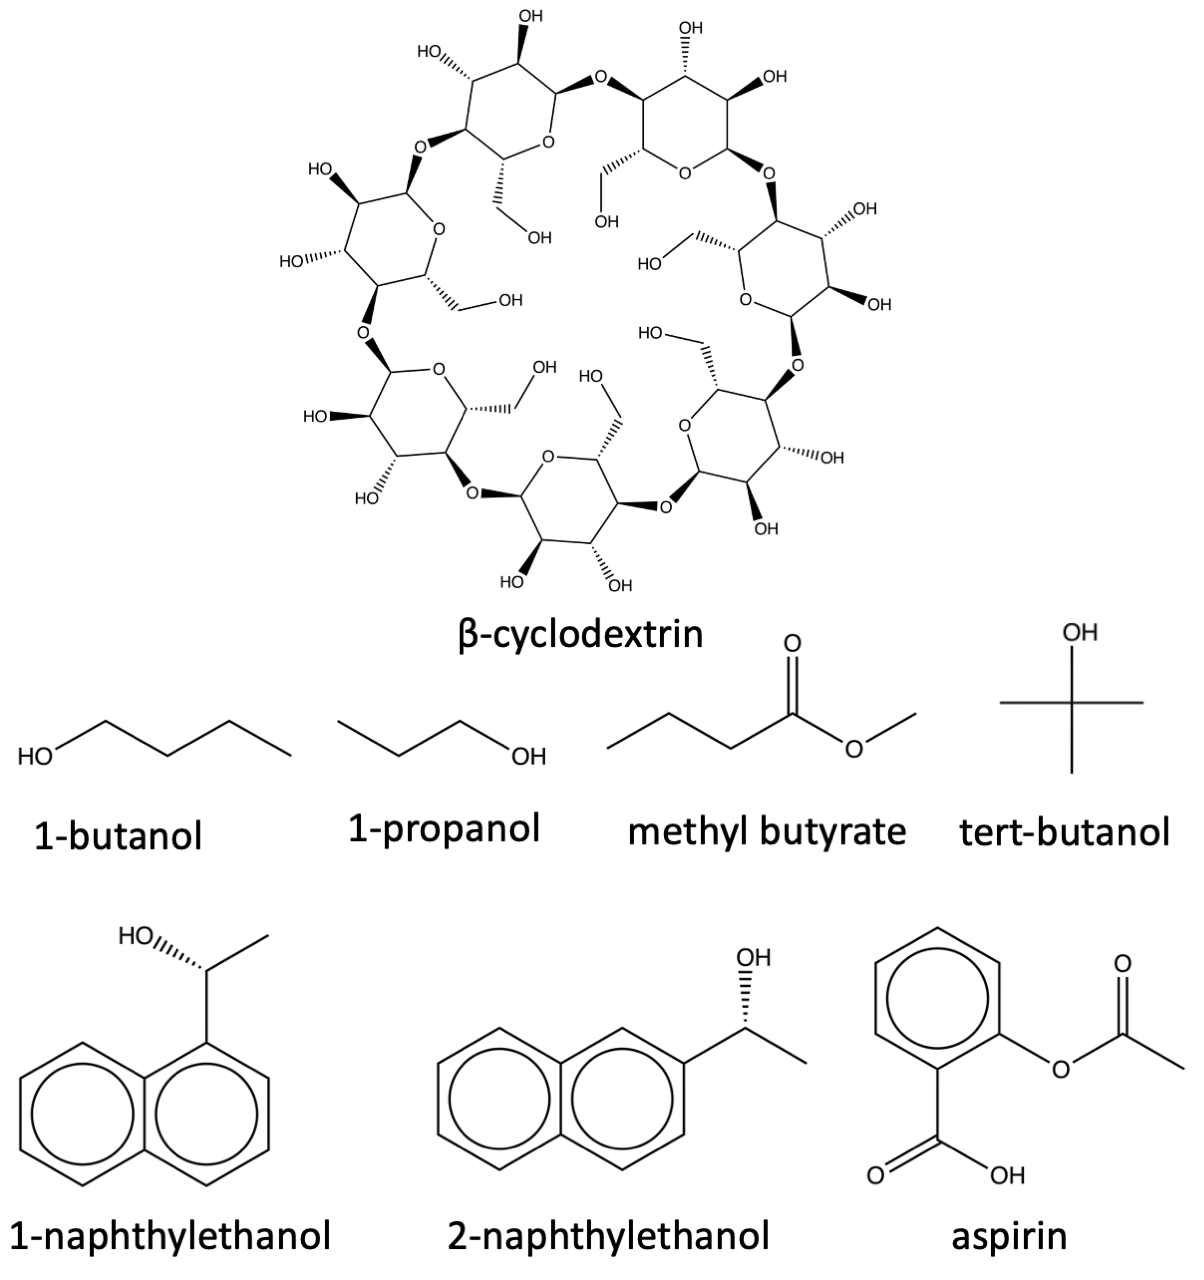
\includegraphics[scale=0.45]{images/figure4.png} 
\caption{$\beta$-cyclodextrin (host) and the seven ligand (guest) molecules}
\label{figure4}
\end{figure} 

\noindent Outline 2 shows the files we will require for the successful completion of the SEEKR2 tutorial on the host-guest complexes.

\vspace{2mm}
\noindent \textbf{2. Preparing PQR files for Brownian dynamics simulations} \par
\vspace{2mm}

\noindent Given the \textit{hostguest.pdb} file containing the receptor ($\beta$-cyclodextrin) and the ligand molecule, we will obtain separate PQR files for the receptor and ligand molecule, respectively. These files are required to run BD simulations to calculate the receptor-ligand binding rates (k\textsubscript{on}). To obtain the PQR files, we will use the ambpdb program integrated into the Ambertools. The ambpdb program requires a topology file (\textit{hostguest.parm7}) and a coordinate file (\textit{hostguest.inpcrd}) to create a PQR file (\textit{hostguest.pqr}). The PQR file is almost identical to a PDB file, except the charge and radius columns in the PQR files substitute the beta and occupancy columns in the PDB file. Once a \textit{hostguest.pqr} file is created using the ambpdb tool, we want to create two separate PQR files from the \textit{hostguest.pqr} file, i.e., the \textit{receptor.pqr} file containing the coordinate, charge, and radius information of the receptor atoms and the \textit{ligand.pqr} file containing the coordinate, charge, and radius information of the ligand atoms. \par

\noindent The python script, \textit{create$\_$BD$\_$files.py} generates a coordinate file, i.e., \textit{hostguest.inpcrd} using the CPPTRAJ module with the structure and topology files as input. \noindent The script then further creates \textit{receptor.pqr} and \textit{ligand.pqr} files by reading into the \textit{hostguest.pqr} file. To achieve this, we execute the following command in the terminal:

\begin{tcolorbox}[colback=black!8!white, colframe=black!50!black, fontlower=\tiny, left=2pt, right=2pt, top=2pt, bottom=2pt] 
\texttt{python create$\_$BD$\_$files.py}
\end{tcolorbox}

\vspace{2mm}
\begin{tcolorbox}[colback=black!8!white, colframe=black!50!black, fontlower=\tiny, left=2pt, right=2pt, top=2pt, bottom=2pt] 
\begin{center}
\noindent \textbf{Outline 2: Overview of the beta$\_$cyclodextrin$\_$guest$\_$ \linebreak complexes directory within working$\_$examples directory}
\end{center}
\begin{forest}
  for tree={
    font=\ttfamily,
    grow'=0,
    child anchor=west,
    parent anchor=south,
    anchor=west,
    calign=first,
    edge path={
      \noexpand\path [draw, \forestoption{edge}]
      (!u.south west) +(7.5pt,0) |- node[fill,inner sep=1.25pt] {} (.child anchor)\forestoption{edge label};
    },
    before typesetting nodes={
      if n=1
        {insert before={[,phantom]}}
        {}
    },
    fit=band,
    before computing xy={l=15pt},
  }
[beta$\_$cyclodextrin$\_$guest$\_$complexes
  [BCD$\_$1-butanol
    [hostguest.pdb]
    [hostguest.parm7]
    [create$\_$BD$\_$files.py]
    [input$\_$SMD$\_$HIDR.xml]
  ]
    [BCD$\_$1-napthylethanol]
    [BCD$\_$1-propanol]
    [BCD$\_$2-napthylethanol]
    [BCD$\_$aspirin]
    [BCD$\_$methyl$\_$butyrate]
    [BCD$\_$terbutanol]
]
\end{forest}
\end{tcolorbox}

\noindent Once the coordinate file is generated, the script then creates a PQR file, i.e., \textit{hostguest.pqr} by executing the following command in the terminal:

\begin{tcolorbox}[colback=black!8!white, colframe=black!50!black, fontlower=\tiny, left=2pt, right=2pt, top=2pt, bottom=2pt] 
\texttt{ambpdb -p hostguest.parm7 -c hostguest.inpcrd \textbackslash \linebreak -pqr > hostguest.pqr}
\end{tcolorbox}

\noindent The Browndye2 software lumps all the charges of the residue into one point charge, which may be acceptable for a protein, as in the case of the \textit{receptor.pqr} file where all the atoms of a particular residue have the same numbering. But for a small ligand, the accuracy can be further improved if we consider each atom as a point charge. This is accomplished by renumbering the atoms of the ligand, each with a different number. To achieve this, we execute the following command in the terminal:

\begin{tcolorbox}[colback=black!8!white, colframe=black!50!black, fontlower=\tiny, left=2pt, right=2pt, top=2pt, bottom=2pt] 
\texttt{python $\sim$/$\$$PWD/scripts/pqr$\_$resid$\_$for$\_$each$\_$atom.py \textbackslash \linebreak ligand.pqr ligand.pqr} \\
\texttt{ $\#$ where $\$$PWD is seekrtools/seekrtools/scripts} 
\end{tcolorbox}

\noindent Now, we have the required files to proceed to the next step. 

\vspace{2mm}
\noindent \textbf{3. Running Steered MD simulations to obtain starting structures for SEEKR2 simulations} \par
\vspace{2mm}

\noindent Determining the anchor points for the host-guest complex is the first step towards milestoning simulations in the SEEKR2 framework. We first choose an appropriate collective variable (CV) to determine the anchor points that could describe the receptor-ligand binding and unbinding dynamics. In the case of the host-guest complex, we choose the distance between the center of mass (COM) of the receptor ($\beta$-cyclodextrin) and the ligand as the CV to determine the anchor points. The anchor points, therefore, lie on a line composed of the COM-COM distance. Once the anchor points are determined, we define concentric spherical milestones around the receptor-ligand binding site where the concentric radii are midpoints of any two consecutive anchor points. These milestones will act as reference points during the simulation. We then use steered MD (SMD) to slowly pull the ligand away from the binding site with a harmonic restraint and save the trajectory snapshots as it crosses the anchor point while slowly moving out of the binding pocket. Once the ligand is pulled out completely, we have the saved structure files, which will be used to create a SEEKR2 file tree where SEEKR2 simulations will occur.  \par

\noindent Holo insertion by directed restraints (HIDR), a computational method employed in the SEEKR2 framework, utilizes one or more initial configurations alongside a SEEKR2 input XML file, pulls the system towards all the anchors present in the SEEKR2 framework until starting structures exist in all of them. The HIDR algorithm employs SMD simulations to accomplish this. \par

\noindent The HIDR program needs a \textit{model.xml} file to run the SMD simulations, so we run the \textit{prepare.py} script on a model input file. The model input XML file for SEEKR2 calculations contains various parameters and settings that define the configuration and behavior of the calculation (Summary 1).  It should be noted that the <md$\_$steps$\_$per$\_$anchor> tag defines the number of MD simulation steps per anchor, and for tutorial purposes, the simulation steps in each anchor are reduced compared to our original study. The <root$\_$directory> tag has to be explicitly defined by the user in the \textit{input$\_$SMD$\_$HIDR.xml} file. To run the prepare.py script on the model input file, we execute the following command in the terminal:

\begin{tcolorbox}[colback=black!8!white, colframe=black!50!black, fontlower=\tiny, left=2pt, right=2pt, top=2pt, bottom=2pt] 
\texttt{python $\sim$/seekr2/seekr2/prepare.py \textbackslash \linebreak input$\_$SMD$\_$HIDR.xml}
\end{tcolorbox}


\begin{mdframed}[backgroundcolor=black!8!white, linewidth=0.5pt, leftmargin=0pt, rightmargin=10pt, innertopmargin=2pt, innerbottommargin=2pt]
%\begin{tcolorbox}[colback=black!8!white, colframe=black!50!black, fontlower=\tiny, left=0pt, right=10pt, top=2pt, bottom=2pt]
\textbf{Summary 1: Overview of sections and tags within the XML file}

\vspace{2mm}
\begin{itemize}[nosep] 
\item \textbf{<calculation$\_$type>}: Specifies the type of milestoning model to employ. SEEKR2 either employs the "mmvt" (Markovian milestoning with Voronoi Tesselations) or the "elber" model for the original Elber milestoning method.
\item \textbf{<calculation$\_$settings>}: A block of settings specific to the chosen calculation type. The tags within this section vary depending on the calculation type.
\item \textbf{<md$\_$output$\_$interval>}: Interval between outputs of simulation state information, trajectory frames, and restart checkpoints (in MD timesteps).
\item \textbf{<md$\_$steps$\_$per$\_$anchor>}: Total number of MD timesteps to be run per anchor.
\item \textbf{<temperature>}: Temperature (in Kelvin) to be used for all stages of the calculation.
\item \textbf{<pressure>}: Pressure (in bar) for simulations if the ensemble is set to npt. Ignored if the ensemble is set to nvt.
\item \textbf{<ensemble>}: Defines the ensemble of MD simulations. Options include nvt (constant volume and temperature) and npt (constant pressure and temperature).
\item \textbf{<root$\_$directory>}: Filesystem path to the directory where the calculation files will be written.
\item \textbf{<md$\_$program>}: Specifies the MD simulation engine to use. The user has the option to choose either openmm or namd.
\item \textbf{<constraints>}: Specifies the type of bond and angle constraints in the MD simulation.
\item \textbf{<rigid$\_$water>}: Specifies whether water molecules will have a rigid angle.
\item\textbf{ <hydrogen$\_$mass>}: Mass (in AMU) to use for hydrogen mass repartitioning (HMR).
\item \textbf{<integrator$\_$type>}: Type of integrator to be used for simulation dynamics.
\item \textbf{<timestep>}: MD timestep (in \SI{}{\pico\second}).
\item \textbf{nonbonded$\_$cutoff}: Nonbonded cutoff (in \SI{}{\nano\meter}) for MD simulations.
\item \textbf{<cv$\_$inputs>}: Settings defining the collective variables (CVs) and their associated anchors and milestones.
\item \textbf{<cv$\_$input>}: Input structure for a CV, with the CV type defined by the class attribute.
\item\textbf{ <group>}: Lists of atom indices for CV functions involving centers of masses of groups of molecules.
\item\textbf{ <bd$\_$group>}: Atoms within PQR files used in BD simulations to define the CV.
\item \textbf{<input$\_$anchors>}: Block of input anchors used to construct model anchors.
\item \textbf{<input$\_$anchor>}: Input for an anchor, with the class attribute matching a particular CV. Attributes depend on the anchor type, such as <starting$\_$amber$\_$params>, <radius>, <lower$\_$milestone$\_$radius>, <upper$\_$milestone$\_$ra \linebreak dius>, etc.
\item \textbf{<browndye$\_$settings$\_$input>} (optional): Settings for Browndye simulations and k\textsubscript{on} calculations.
\item \textbf{<binary$\_$directory>}: Directory containing Browndye2 programs
\item \textbf{<receptor$\_$pqr$\_$filename>}: Path to the PQR file representing the receptor.
\item \textbf{<ligand$\_$pqr$\_$filename>}: Path to the PQR file representing the ligand.
\item \textbf{<apbs$\_$grid$\_$spacing>}: Grid spacing (in \SI{}{\angstrom}) for APBS calculations.
\item\textbf{ <receptor$\_$indices}>: Atom indices defining the binding site in the receptor PQR file.
\item \textbf{<ligand$\_$indices>}: Atom indices defining the center of the ligand molecule in the ligand PQR file.
\item \textbf{<ions>}: Block of ion objects used in APBS and BD calculations.
\item \textbf{<ion>}: Object representing an ion with attributes like <radius>, <charge>, and <conc>.
\item \textbf{<num$\_$b$\_$surface$\_$trajectories>}: Total number of trajectories for b-surface simulations.
\item \textbf{<n$\_$threads}>: Number of CPUs to use in Browndye2 calculations.
\end{itemize}
\end{mdframed}
%\end{tcolorbox}
\vspace{2mm}

\noindent Now the model XML file and the SEEKR2 file tree have been generated in a separate \textit{SEEKR$\_$simulation} directory as specified explicitly by the <root$\_$directory> tag in the model input XML file, i.e., the \textit{input$\_$SMD$\_$HIDR.xml} file. HIDR will now employ SMD simulations to gradually pull the system into every anchor and save the structures for subsequent SEEKR2 calculations. It is important to note that HIDR offers alternative approaches, such as random acceleration MD (RAMD) and ratcheting, to populate starting structures. For detailed instructions on utilizing these alternative methods, it is recommended to refer to the HIDR documentation and seekrtools tutorials. To run SMD simulations with the HIDR algorithm, execute the following command in the terminal:

\begin{tcolorbox}[colback=black!8!white, colframe=black!50!black, fontlower=\tiny, left=2pt, right=2pt, top=2pt, bottom=2pt] 
\texttt{python $\sim$/seekrtools/seekrtools/hidr/hidr.py \textbackslash \linebreak any SEEKR$\_$simulation/model.xml -M SMD -p \textbackslash \linebreak hostguest.pdb}
\end{tcolorbox}

\noindent This command is likely to run for hours or days, depending on the speed of the GPU. We can obtain a comprehensive overview of HIDR arguments by executing HIDR with the -h argument using the following python command:

\begin{tcolorbox}[colback=black!8!white, colframe=black!50!black, fontlower=\tiny, left=2pt, right=2pt, top=2pt, bottom=2pt] 
\texttt{python $\sim$/seekrtools/seekrtools/hidr/hidr.py -h}
\end{tcolorbox}

\noindent Several important options are available, such as specifying the number of equilibration steps to be executed before SMD simulations. For example, including the argument below will instruct HIDR to perform 5,000,000 equilibration steps (10 ns) before initiating any SMD simulations:

\begin{tcolorbox}[colback=black!8!white, colframe=black!50!black, fontlower=\tiny, left=2pt, right=2pt, top=2pt, bottom=2pt] 
\texttt{python $\sim$/seekrtools/seekrtools/hidr/hidr.py \textbackslash \linebreak any SEEKR$\_$simulation/model.xml -M SMD -p \textbackslash \linebreak hostguest.pdb -e 5000000}
\end{tcolorbox}

\noindent Additionally, we can allow for some equilibration steps within each anchor after the SMD simulation has reached that particular anchor. These equilibration steps are referred to as settling steps in HIDR. To specify the number of settling steps, the -S argument is used. To allow for 200,000 settling steps (0.2 ns), we execute the following command in the terminal:

\begin{tcolorbox}[colback=black!8!white, colframe=black!50!black, fontlower=\tiny, left=2pt, right=2pt, top=2pt, bottom=2pt] 
\texttt{python $\sim$/seekrtools/seekrtools/hidr/hidr.py \textbackslash \linebreak any SEEKR$\_$simulation/model.xml -M SMD -p \textbackslash \linebreak hostguest.pdb -S 100000}
\end{tcolorbox}

\noindent By default, HIDR SMD simulations move the system towards each anchor at an approximate 0.01 nm/ns speed. This speed is designated to let the system reach each anchor within a reasonable time frame while avoiding excessive perturbations to the system. However, the speed can be adjusted using the -v argument. For instance, if the user desires to perform SMD simulations ten times faster (thus completing in one-tenth of the time), the speed can be set to 0.1 nm/ns:

\begin{tcolorbox}[colback=black!8!white, colframe=black!50!black, fontlower=\tiny, left=2pt, right=2pt, top=2pt, bottom=2pt] 
\texttt{python $\sim$/seekrtools/seekrtools/hidr/hidr.py \textbackslash \linebreak any SEEKR$\_$simulation/model.xml -M SMD -p \textbackslash \linebreak hostguest.pdb -v 0.1}
\end{tcolorbox}

\noindent To keep the directory clean, we can optionally choose to delete the intermediate files:

\begin{tcolorbox}[colback=black!8!white, colframe=black!50!black, fontlower=\tiny, left=2pt, right=2pt, top=2pt, bottom=2pt] 
\texttt{rm hostguest.inpcrd hostguest.pqr ligand.pqr \textbackslash \linebreak receptor.pqr}
\end{tcolorbox}


\subsection*{Stage 2: Run}
\vspace{2mm}

\noindent During the prepare stage of a SEEKR2 calculation, a file tree containing all the necessary files and directories is generated at the specified location indicated by the <root$\_$directory> tag in the model input file. Once the preparation stage is complete, we move on to the run stage. 

\noindent The run stage involves executing the simulations based on the files and directories from the prepare stage. Inside this directory, i.e., \textit{SEEKR$\_$simulation}, a \textit{model.xml} file exists. In the subsequent stages of SEEKR2, especially the run stage and beyond, the path to the \textit{model.xml} file is used as an argument in most SEEKR2 programs. It is important to note that modifying the \textit{model.xml} file directly without re-running the \textit{prepare.py} script is not recommended. To start the run stage, we will use the \textit{run.py} script. The following command launches the script to run MD simulations within the SEEKR2 milestones:

\begin{tcolorbox}[colback=black!8!white, colframe=black!50!black, fontlower=\tiny, left=2pt, right=2pt, top=2pt, bottom=2pt] 
\texttt{python $\sim$/seekr2/seekr2/run.py any \textbackslash \linebreak SEEKR$\_$simulation/model.xml}
\end{tcolorbox}

\noindent In the above command, the word "any" is the instruction argument for the \textit{run.py} script. It instructs the script to run any unfinished MD or BD simulations. We can use "any$\_$md" or "any$\_$bd"  as an instruction input to run only unfinished MD or BD simulations. Please refer to the SEEKR2 documentation for a comprehensive list of available instruction inputs as \textit{run.py} arguments.

\noindent Once we initiate the \textit{run.py} script, simulations will run until completion or interruption. The SEEKR2 framework saves checkpoints for both MD and BD simulations, allowing us to resume the calculation from where it was interrupted. To track the progress and convergence of the simulations, we  use the \textit{converge.py} script:

\begin{tcolorbox}[colback=black!8!white, colframe=black!50!black, fontlower=\tiny, left=2pt, right=2pt, top=2pt, bottom=2pt] 
\texttt{python $\sim$/seekr2/seekr2/converge.py any \textbackslash \linebreak SEEKR$\_$simulation/model.xml}
\end{tcolorbox}

\noindent Running the \textit{converge.py} script generates convergence plots, and images are saved in the \textit{plots$\_$and$\_$images} subfolder within the <root$\_$directory>. For additional arguments that can be used with both \textit{run.py} and \textit{converge.py}, we can run either script with the -h argument (Summary 2). 


\begin{tcolorbox}[colback=black!8!white, colframe=black!50!black, fontlower=\tiny, left=0pt, right=10pt, top=2pt, bottom=2pt]
\textbf{Summary 2: Arguments for converge.py}

\vspace{2mm}

\noindent \textbf{Positional Arguments} \par

\begin{itemize}

\item \textbf{MODEL$\_$FILE}: This argument specifies the name of the model file for the SEEKR2 calculation. We need to replace \texttt{MODEL$\_$FILE} with the model file name, i.e., \textit{model.xml} used in the calculation.

\end{itemize}

\vspace{2mm}

\noindent \textbf{Optional Arguments} \par

\begin{itemize}

\item \textbf{-s K$\_$ON$\_$STATE}: This argument allows us to define the bound state used to compute the k\textsubscript{on} value. If we want to specify a particular bound state, we include the -s option followed by the state name.

\item \textbf{-d IMAGE$\_$DIRECTORY}: Using this argument, we can define the directory where plots and images will be saved. If we want to specify a different directory, we include the -d option followed by the desired directory path. By default, all the plots will be saved to the \textit{images$\_$and$\_$plots} directory. 

\item \textbf{-c CUTOFF}: This argument sets the minimum convergence value required to conclude that the calculations have converged for a given anchor. The default value is 0.1, but we can specify a different cutoff value by including the -c option followed by the desired value.

\item \textbf{-m MINIMUM$\_$ANCHOR$\_$TRANSITIONS}: Using this argument, we can set the minimum number of transitions that must be observed per milestone in a given anchor as a criterion for SEEKR2 simulations. The default value is 100, but we can specify a different value by including the -m option followed by the desired number.

\item \textbf{-l, --long$\_$converge}: This argument determines whether to run a complete convergence analysis. Including the -l flag in the command will enable the extended convergence analysis. By default, this is set to False.

\end{itemize}
\end{tcolorbox}


\subsection*{Stage 3: Analyze}
\vspace{2mm}

\noindent The final stage within the SEEKR2 framework involves analyzing the results obtained from the simulations. This stage enables the construction of kinetics and thermodynamics profiles for the studied process.

\begin{tcolorbox}[colback=black!8!white, colframe=black!50!black, fontlower=\tiny, left=0pt, right=10pt, top=2pt, bottom=2pt]

\textbf{Summary 3: Arguments for analyze.py}

\vspace{2mm}

\noindent \textbf{Positional Arguments} \par
\begin{itemize}

\item \textbf{MODEL$\_$FILE}: This argument specifies the name of the model file for the SEEKR2 calculation. We need to replace \texttt{MODEL$\_$FILE} with the model file name, i.e., \textit{model.xml} used in the calculation.

\end{itemize}

\vspace{2mm}

\noindent \textbf{Optional Arguments} \par

\begin{itemize}

\item \textbf{-f, --force\_warning}: By default, missing statistics for any anchors will generate fatal errors. This option will instead raise a warning and attempt the calculation anyway.

\item \textbf{-n NUM\_ERROR\_SAMPLES}: This argument specifies the number of error samples to generate for estimating the error/uncertainty of computed values. The default value is 100.

\item \textbf{-S STRIDE\_ERROR\_SAMPLES}: This argument specifies the number of strides between saved error samples. An argument of \textit{None} automatically assigns the quantity at the number of milestones in the model squared. The default value is None.

\item \textbf{-K SKIP\_ERROR\_SAMPLES, --skip\_error\_samples SKIP\_ERROR\_SAMPLES}: This argument specifies the number of error samples to skip before using them. An argument of None automatically assigns the quantity at ten times the number of milestones in the model squared. The default value is None.

\item \textbf{-d IMAGE\_DIRECTORY}: By using this argument, we can define the directory where plots and images will be saved. If we want to specify a different directory, we include the -d option followed by the desired directory path. By default, all the plots will be saved to the \textit{images$\_$and$\_$plots} directory. 

\item \textbf{-s, --skip\_checks}: By default, post-simulation checks will be run before the analysis is started, and if the checks fail, the analysis will not proceed. This argument bypasses those checks and allows the analysis to proceed anyways.

\item \textbf{-t MINIMUM\_TIME}: A user may wish to skip a simulation time for each anchor before counting the transitions for milestoning analysis. When performing analysis, we enter the time (in ps) to skip a portion of the production simulations.

\item \textbf{-T MAXIMUM\_TIME, --maximum\_time MAXIMUM\_TIME}: A user may wish to stop the analysis of simulation time for each anchor at a particular time. We enter the time (in ps) to end the analysis at a given anchor if the simulation time exceeds it.

\end{itemize}
\end{tcolorbox}




\vspace{2mm}
\noindent To execute the post-simulation SEEKR2 analysis:

\begin{tcolorbox}[colback=black!8!white, colframe=black!50!black, fontlower=\tiny, left=2pt, right=2pt, top=2pt, bottom=2pt] 
\texttt{python $\sim$/seekr2/seekr2/analyze.py  \textbackslash \linebreak SEEKR$\_$simulation/model.xml}
\end{tcolorbox}

\noindent The \textit{analyze.py} script takes the \textit{model.xml} file as an argument. It constructs the milestoning model, populates it with transition probabilities and simulation times within each milestone, and computes error margins. For a list of arguments that can be used with \textit{analyze.py}, we can run the script with the -h argument (Summary 3). Figure \ref{figure5} shows the free energy profile per milestone for the BCD-1-butanol complex, obtained by executing the \textit{analyze.py} script.


\begin{figure}[H]
\centering
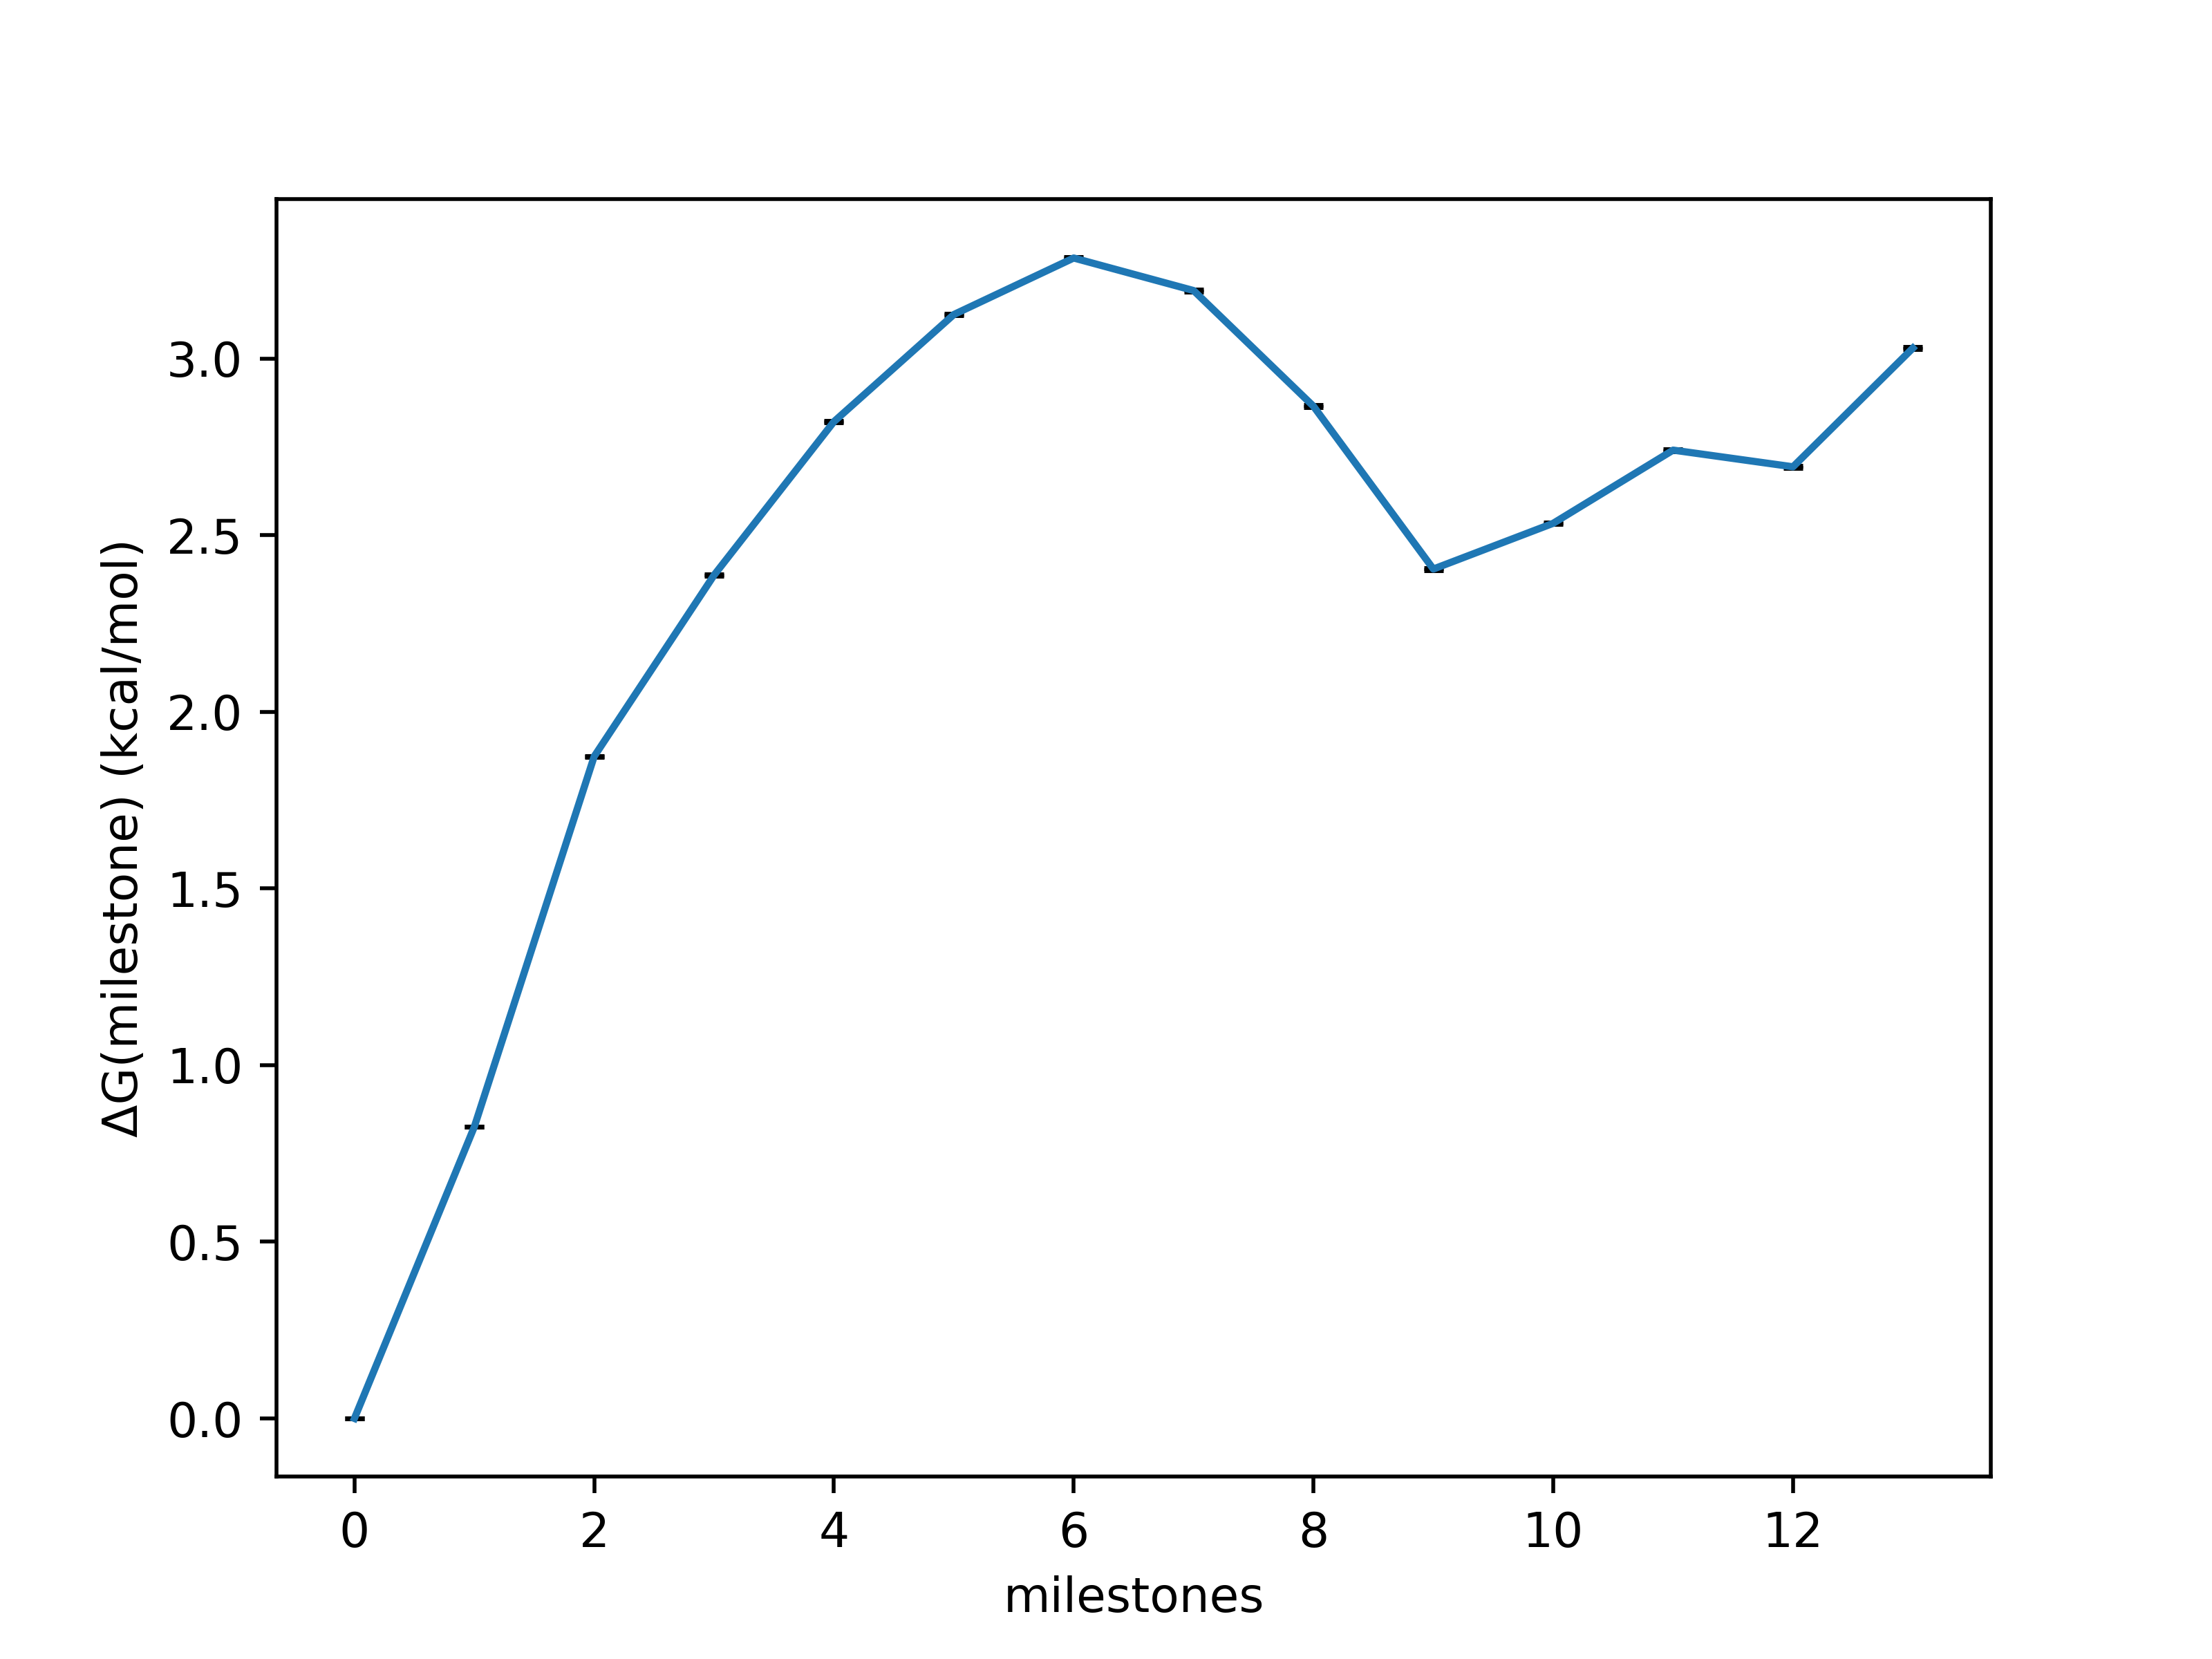
\includegraphics[scale=0.60]{images/figure5.png} 
\caption{Free energy profile per milestone ($\Delta$G\textsubscript{i}) obtained from the SEEKR2 milestoning method for the $\beta$-cyclodextrin (host) and the 1-butanol (guest) complex.}
\label{figure5}
\end{figure} 

\subsection{Advanced Tutorial: Trypsin-benzamidine complex} \label{tryp_ben}
\vspace{2mm}

\subsection*{Stage 1: Prepare}
\vspace{2mm}

\noindent \textbf{1. Obtaining the structure and the parameter file for the trypsin-benzamidine complex} \par
\vspace{2mm}

\noindent This section will prepare input files for the SEEKR2 simulation to determine the (un)binding kinetics between the receptor protein, trypsin, and the ligand molecule, benzamidine. The Amber molecular mechanics forcefield is used to parameterize the receptor-ligand complex. This tutorial assumes the user has some familiarity with AmberTools. If the user is new to AmberTools, we recommend visiting the Amber tutorials page (\ambertutorialslink) or reviewing the Amber manual (\ambermanuallink) for a comprehensive understanding. Outline 3 shows the files we will require for the successful completion of the SEEKR2 tutorial on the trypsin-benzamidine complex.

\vspace{2mm}
\noindent \textbf{(i) Identify the ligand molecule and the receptor protein in the receptor-ligand complex} \par
\vspace{2mm}
\noindent The first step is to identify the molecules in the receptor-ligand complex. In this case, we have trypsin as the target molecule and benzamidine as the ligand molecule. The trypsin-benzamidine complex is a standard complex for studying binding and unbinding kinetics.

\vspace{2mm}
\noindent \textbf{(ii) Parameterization of the receptor-ligand complex} \par

\noindent In the SEEKR2 framework, to estimate the binding and unbinding of receptor-ligand bimolecular complexes, one of the molecules is the ligand that needs to be parameterized separately. One method to accomplish this is to use the Antechamber program in AmberTools. Antechamber requires a structure file specific to the small molecule to perform the parameterization. In our case, we will utilize a PDB file that contains only the benzamidine structure, which has been parametrized using a semi-empirical method and the generalized AMBER force field. Although semi-empirical methods for assigning charges are quick and convenient, they may not provide the most accurate results for assigning partial charges to a molecule. It is advisable to explore more precise levels of quantum calculations to obtain partial charges, such as Hartree Fock with Density Function Theory (HF-DFT) or Møller-Plesset 2 (MP2) calculations within a charge model such as RESP or CHELPG. However, these calculations involving higher levels of quantum theory require dedicated quantum calculation software like Gaussian, GAMESS, ORCA, etc. Incorporating parameters from quantum calculation software is a complex topic that is beyond the scope of this tutorial. \par

\vspace{2mm}
\begin{tcolorbox}[colback=black!8!white, colframe=black!50!black, fontlower=\tiny, left=2pt, right=2pt, top=2pt, bottom=2pt] 
\begin{center}
\noindent \textbf{Outline 3: Overview of the trypsin$\_$benzamidine$\_$ \linebreak complex directory within working$\_$examples directory}
\end{center}
\begin{forest}
  for tree={
    font=\ttfamily,
    grow'=0,
    child anchor=west,
    parent anchor=south,
    anchor=west,
    calign=first,
    edge path={
      \noexpand\path [draw, \forestoption{edge}]
      (!u.south west) +(7.5pt,0) |- node[fill,inner sep=1.25pt] {} (.child anchor)\forestoption{edge label};
    },
    before typesetting nodes={
      if n=1
        {insert before={[,phantom]}}
        {}
    },
    fit=band,
    before computing xy={l=15pt},
  }
[trypsin$\_$benzamidine$\_$complex
  [hostguest.pdb]
  [minimize$\_$equilibriate.py]
  [extract$\_$benzamidine.py]
  [create$\_$BD$\_$files.py]
  [parameterize$\_$trypsin$\_$benzamidine.tleap]
  [save$\_$benzamidine$\_$lib.tleap]
  [input$\_$SMD$\_$HDR.xml]
  ]
]
\end{forest}
\end{tcolorbox}

\noindent To save a separate PDB structure of the ligand molecule (\textit{benzamidine.pdb}) from the given receptor-ligand complex (\textit{trypsin$\_$benzamidine$\_$init.pdb}), we execute the following command in the terminal. 

\begin{tcolorbox}[colback=black!8!white, colframe=black!50!black, fontlower=\tiny, left=2pt, right=2pt, top=2pt, bottom=2pt] 
\texttt{python extract\_benzamidine.py}
\end{tcolorbox}

\noindent We use the Antechamber program, part of AmberTools to parameterize the benzamidine molecule. The antechamber command takes several arguments to specify input and output files, formats, and parameters (Summary 4). We will execute the following command in the terminal to parameterize the benzamidine molecule. 

\begin{tcolorbox}[colback=black!8!white, colframe=black!50!black, fontlower=\tiny, left=2pt, right=2pt, top=2pt, bottom=2pt] 
\texttt{antechamber -i benzamidine.pdb -fi pdb -bk BEN \textbackslash \linebreak -o benzamidine.mol2 -fo mol2 -c bcc -nc 1} 
\end{tcolorbox}

\noindent We will now generate a parameter modification (frcmod) file containing the molecular force field parameters for the benzamidine molecule. This file is later used in the LEAP functionality of the Ambertools to parameterize the receptor-ligand complex. The ParmChk2 program generates the frcmod file for the benzamidine molecule. We will execute the following command in the terminal to generate the frcmod file. 

\begin{tcolorbox}[colback=black!8!white, colframe=black!50!black, fontlower=\tiny, left=2pt, right=2pt, top=2pt, bottom=2pt]  
\texttt{parmchk2 -i benzamidine.mol2 -f mol2 -o \textbackslash \linebreak benzamidine.frcmod}
\end{tcolorbox}

\begin{figure}[H]
\centering
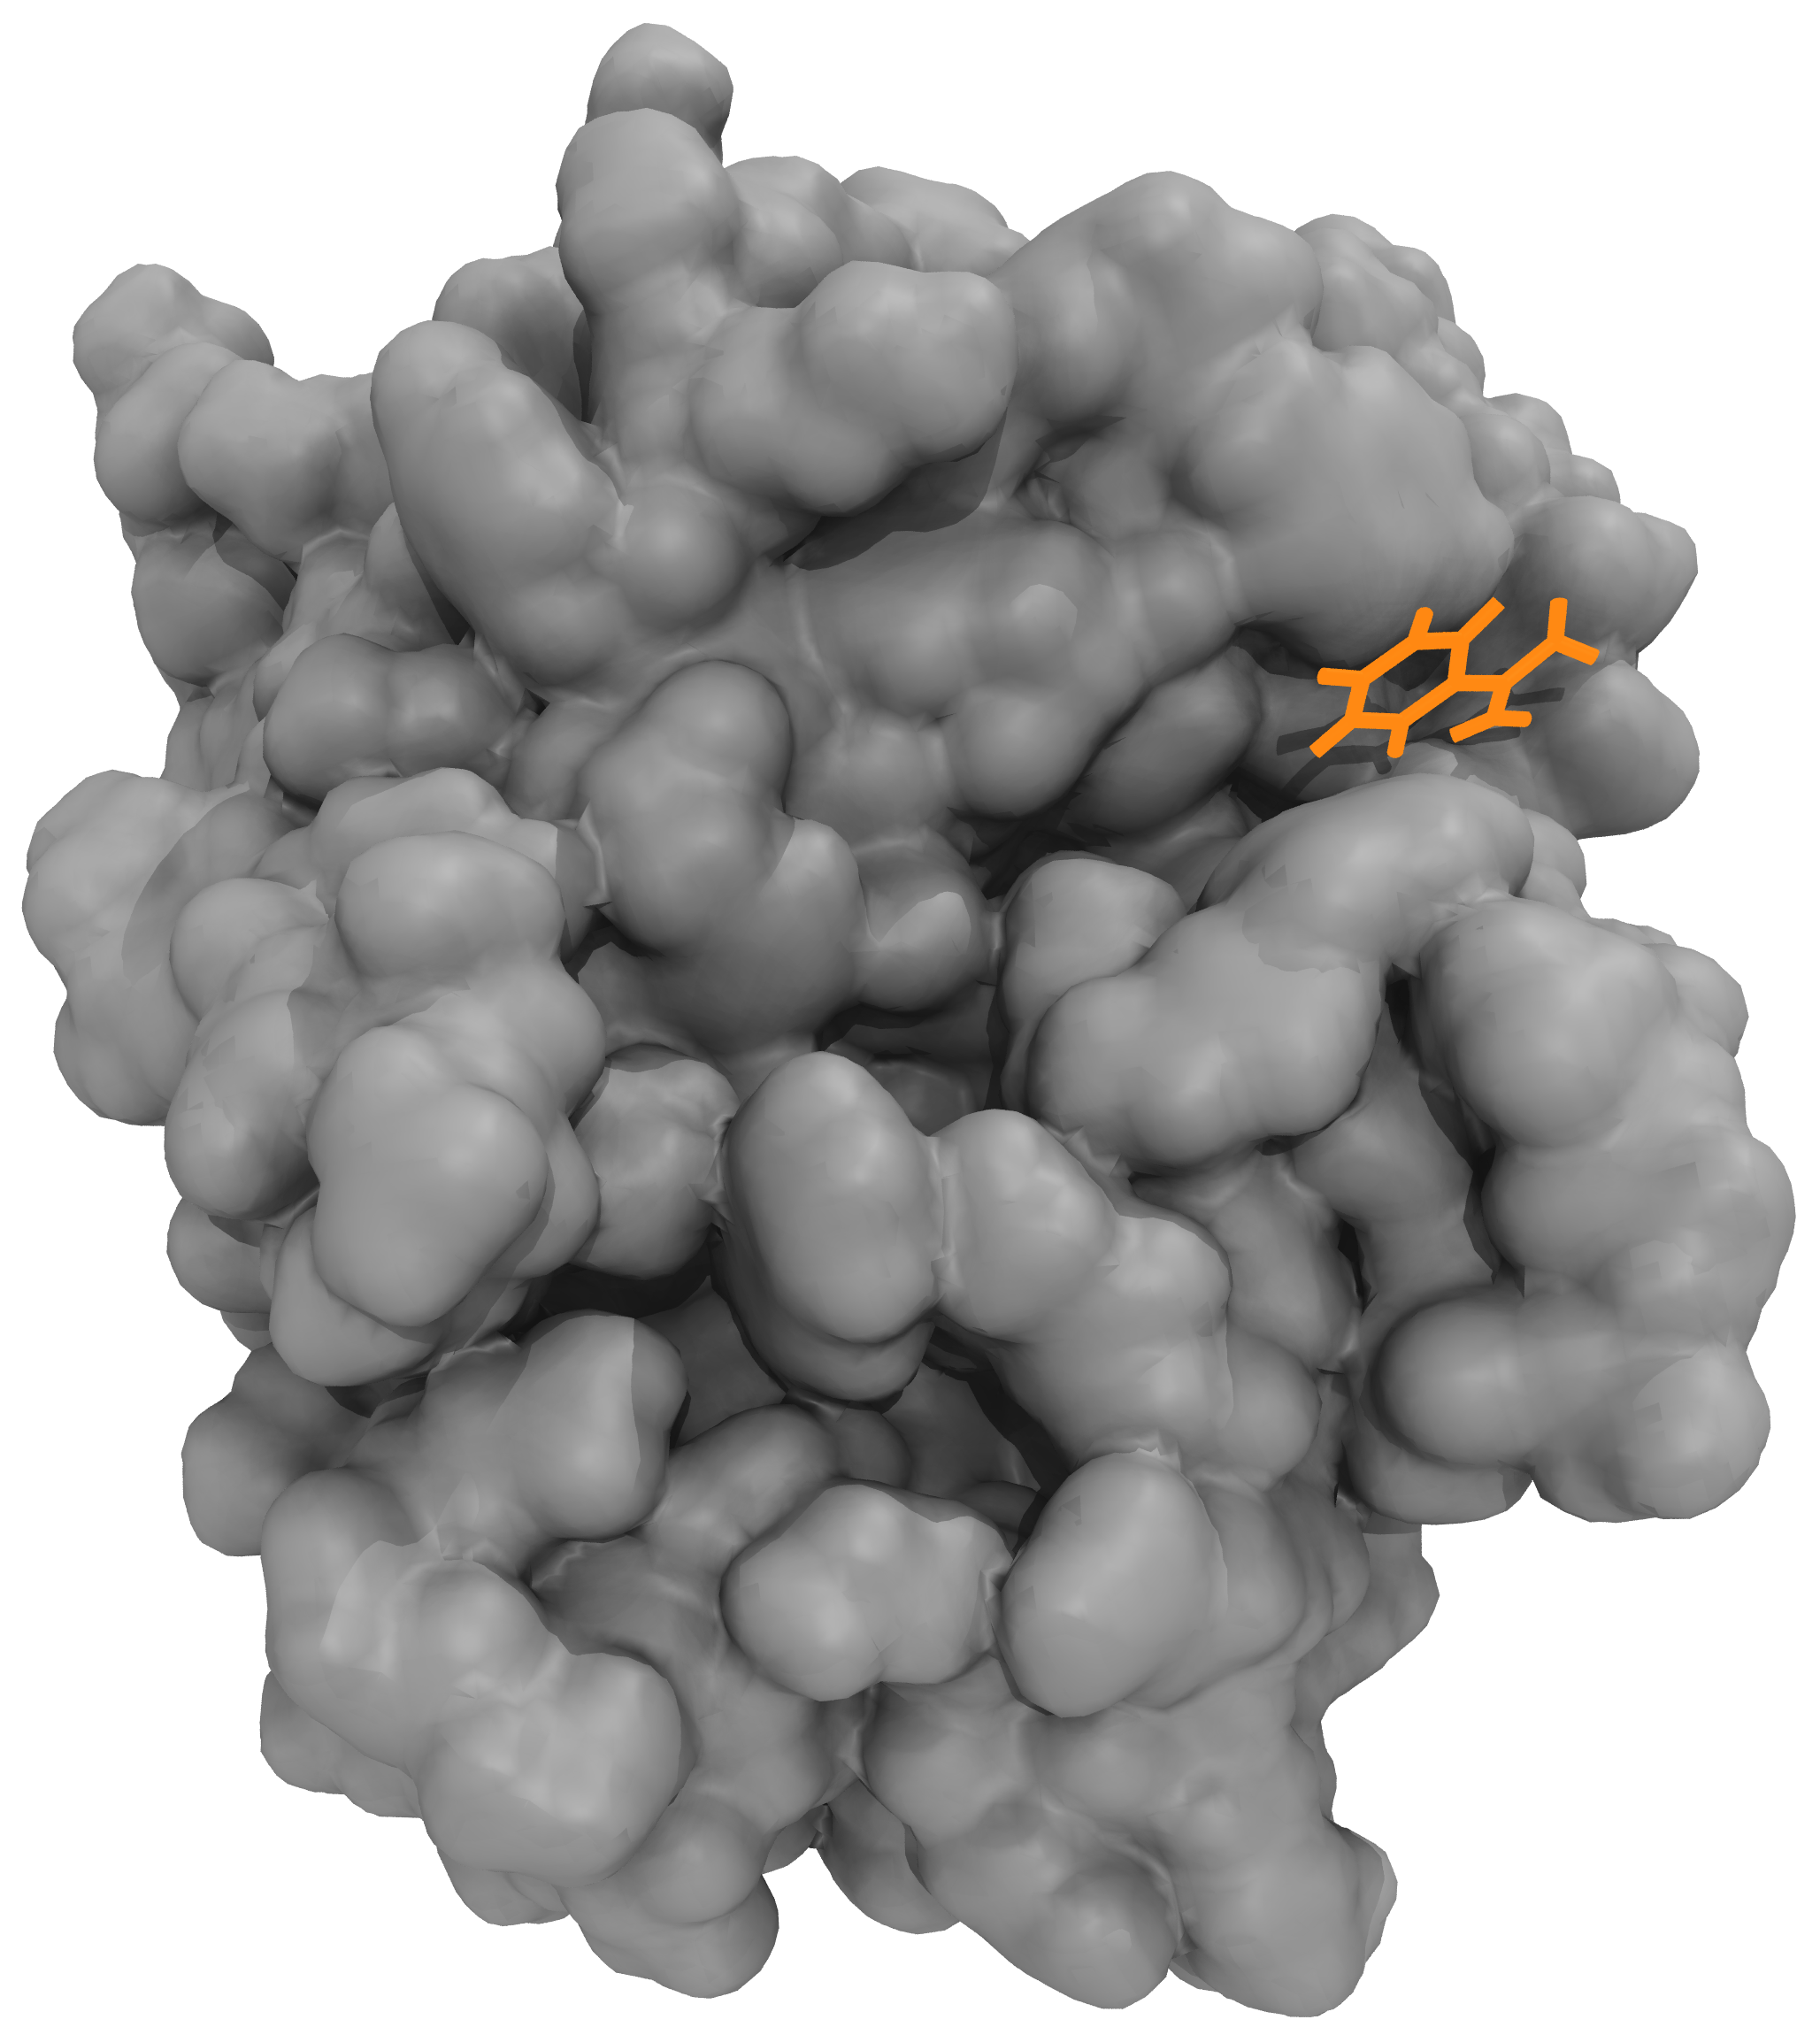
\includegraphics[scale=0.12]{images/figure6.png} 
\caption{Trypsin - benzamidine complex}
\label{figure6}
\end{figure} 

\noindent We generate a .lib file, a library file of forcefield parameters for the benzamidine molecule, by executing the following command in the terminal:

\begin{tcolorbox}[colback=black!8!white, colframe=black!50!black, fontlower=\tiny, left=2pt, right=2pt, top=2pt, bottom=2pt] 
\texttt{tleap -f save$\_$benzamidine$\_$lib.tleap}
\end{tcolorbox}

\noindent The final step in parameterizing the trypsin-benzamidine complex involves solvating the system with water molecules and applying periodic boundary conditions. This ensures that the simulation accurately represents the behavior of the complex in an aqueous environment while accounting for long-range interactions and avoiding edge effects. Additionally, counterions are added to neutralize any net charge in the system, creating an electrically neutral simulation system. We execute the following command in the terminal to parameterize the trypsin-benzamidine complex:

\begin{tcolorbox}[colback=black!8!white, colframe=black!50!black, fontlower=\tiny, left=2pt, right=2pt, top=2pt, bottom=2pt] 
\texttt{tleap -f parameterize$\_$trypsin$\_$benzamidine.tleap}
\end{tcolorbox}

\begin{tcolorbox}[colback=black!8!white, colframe=black!50!black, fontlower=\tiny, left=0pt, right=10pt, top=2pt, bottom=2pt]
\textbf{Summary 4: Arguments used in the antechamber parameterization of the ligand}
\begin{itemize}
\item \texttt{\textbf{-i \textit{benzamidine.pdb}}}: Take the \texttt{ben.pdb} file as input.
\item \texttt{\textbf{-fi pdb}}: The format of \texttt{benzamidine.pdb} is in PDB format.
\item \texttt{\textbf{-bk BEN}}: The component/block ID for benzamidine in the PDB file is \texttt{BEN}.
\item \texttt{\textbf{-o \textit{benzamidine.mol2}}}: Specifies the output file name of the benzamidine molecule.
\item \texttt{\textbf{-fo mol2}}: Outputs the \texttt{benzamidine.mol2} file in MOL2 format.
\item \texttt{\textbf{-c bcc}}: Uses the AM1-BCC semi-empirical method to assign partial charges of the atoms.
\item \texttt{\textbf{-nc 1}}: The molecule has a net molecular charge of +1 due to its protonation state in aqueous environments at pH = 7.
\end{itemize}
\end{tcolorbox}

\noindent In the \textit{parameterize$\_$trypsin$\_$benzamidine.tleap} file, explanations for the commands are as under: 
\begin{itemize}
\item \texttt{\textbf{source leaprc.protein.ff14SB}}: Sourcing the ff14SB forcefield, a recently generated force field parameter set known for its good performance in molecular simulations of proteins, provides accurate descriptions of protein atoms and their interactions.
\item \texttt{\textbf{source leaprc.water.tip4pew}}: By sourcing the leaprc.water.tip4pew file, the TIP4Pew water model is employed. This water model is considered more accurate than the commonly used TIP3P model.
\item \texttt{\textbf{solvateoct receptor$\_$ligand$\_$complex TIP4PEWBOX 8}}: This command solvates the receptor-ligand complex, represented by the variable receptor$\_$ligand$\_$complex, in a truncated octahedral box using TIP4Pew water molecules. The truncated octahedral shape is preferred over a simple cubic box due to its more efficient use of space, reducing the number of water molecules required to solvate the system. The specified padding of 8 \SI{}{\angstrom} creates a buffer region around the protein to prevent any artifacts from periodic boundary conditions.
\item \texttt{\textbf{addIons2 mol Cl- 7}}: Since the system has a net positive charge, adding chloride ions (Cl-) neutralizes the overall charge. When setting up simulations, it is generally recommended to carefully consider the ions present in the experimental or physiological conditions to mimic the real environment closely. However, in this specific scenario, the decision to use only chloride ions is based on the information available and the challenges associated with including other ions.
\end{itemize}

\noindent To remove multiple output files generated by the antechamber and leap commands, which are no longer required for subsequent parameterization steps, we can execute the following command in the terminal:

\begin{tcolorbox}[colback=black!8!white, colframe=black!50!black, fontlower=\tiny, left=2pt, right=2pt, top=2pt, bottom=2pt] 
\texttt{rm *ANTECHAMBER* ATOMTYPE.INF *sqm* leap.log \textbackslash \linebreak benzamidine.frcmod benzamidine.lib \textbackslash \linebreak benzamidine.mol2 benzamidine.pdb}
\end{tcolorbox}

\noindent The next step involves the energy minimization of the trypsin-benzamidine complex to its local minima, followed by equilibration in the NVT ensemble. System minimization aims to find an energetically stable conformation of the system by iteratively adjusting the atomic positions to minimize the potential energy, therefore beginning with a favorable starting structure. Equilibration prepares the biomolecular complexes for MD production runs by resolving initial structural and energetic irregularities, ensuring stable and reliable simulations under target conditions. To perform the energy minimization followed by system equilibration, we execute the following command in the terminal:

\begin{tcolorbox}[colback=black!8!white, colframe=black!50!black, fontlower=\tiny, left=2pt, right=2pt, top=2pt, bottom=2pt] 
\texttt{python minimize$\_$equilibriate.py}
\end{tcolorbox}

\vspace{2mm}
\noindent \textbf{2. Preparing PQR files for Brownian dynamics simulations} \par
\vspace{2mm}

\noindent Given the \textit{trypsin$\_$benzamidine.pdb} file containing the receptor (trypsin) protein and the ligand (benzamidine) molecule, we will obtain separate PQR files for the receptor and ligand molecule, respectively. The ambpdb program requires a topology file (\textit{trypsin$\_$benzamidine.prmtop}) and a coordinate file (\textit{trypsin$\_$benzamidine.inpcrd}) to create a PQR file (\textit{trypsin$\_$benzamidine.pqr}). Once a \textit{trypsin$\_$benzamidine.pqr} file is created using the ambpdb tool, we would want to create two separate PQR files from the \textit{trypsin$\_$benzamidine.pqr} file, i.e., the \textit{trypsin.pqr} file containing the coordinate, charge, and radius information of the receptor atoms and the \textit{ benzamidine.pqr} file containing the coordinate, charge, and radius information of the ligand atoms. \par

\noindent The python script, create$\_$BD$\_$files.py generates a coordinate file, i.e., \textit{trypsin$\_$benzamidine.inpcrd} using the CPPTRAJ module with the structure and topology files as input. Once the coordinate file is generated, the script then creates a PQR file, i.e., \textit{trypsin$\_$benzamidine.pqr} by executing the following command:

\begin{tcolorbox}[colback=black!8!white, colframe=black!50!black, fontlower=\tiny, left=2pt, right=2pt, top=2pt, bottom=2pt] 
\texttt{ambpdb -p trypsin$\_$benzamidine.prmtop -c \textbackslash \linebreak trypsin$\_$benzamidine.inpcrd -pqr > \textbackslash \linebreak trypsin$\_$benzamidine.pqr}
\end{tcolorbox}

\noindent The script then further creates \textit{trypsin.pqr} and \textit{benzamidine.pqr} files by reading into the \textit{trypsin$\_$benzamidine.pqr} file. To achieve this, we execute the following command in the terminal:

\begin{tcolorbox}[colback=black!8!white, colframe=black!50!black, fontlower=\tiny, left=2pt, right=2pt, top=2pt, bottom=2pt] 
\texttt{python create$\_$BD$\_$files.py}
\end{tcolorbox}

\noindent \noindent While the Browndye2 software consolidates all residue charges into a single point charge, suitable for proteins like in the case of \textit{trypsin.pqr} file with uniformly numbered atoms within a residue. But for small ligands, accuracy is enhanced by treating each atom as a distinct point charge and renumbering them individually. To achieve this, we execute the following command in the terminal:

\begin{tcolorbox}[colback=black!8!white, colframe=black!50!black, fontlower=\tiny, left=2pt, right=2pt, top=2pt, bottom=2pt] 
\texttt{python $\sim$/$\$$PWD/scripts/pqr$\_$resid$\_$for$\_$each$\_$atom.py \textbackslash \linebreak benzamidine.pqr benzamidine.pqr} \\
\texttt{ $\#$ where $\$$PWD is seekrtools/seekrtools/scripts} 
\end{tcolorbox}


\noindent Now, we have the required files to proceed to the next step. 

\vspace{2mm}
\noindent \textbf{3. Running Steered MD simulations to obtain starting structures for SEEKR2 simulations} \par
\vspace{2mm}

\noindent To determine the anchor points for milestoning simulations in the SEEKR2 framework, we choose the appropriate CV for the trypsin-benzamidine complex. Here, the distance between the center of mass (COM) of the binding site of the trypsin protein and the ligand serves the CV, followed by determining the anchor points (Figure \ref{figure7}). Subsequently, we establish concentric spherical milestones around the binding site, using midpoints between successive anchor points as their radii. Through SMD simulations, the benzamidine ligand is slowly extracted from the binding site, capturing trajectory snapshots at each anchor point. Once the ligand is pulled out entirely and we have the saved structure files, a SEEKR2 file tree is created where SEEKR2 simulations will occur.  \par

\noindent As mentioned previously, the HIDR program requires a \textit{model.xml} file to run the SMD simulations, so we run the \textit{prepare.py} script on a model input file. It should be noted that the  <md$\_$steps$\_$per$\_$anchor> tag defines the number of MD simulation steps per anchor, and for tutorial purposes, the simulation steps in each anchor are reduced. The <root$\_$directory> tag has to be explicitly defined by the user in the \textit{input$\_$SMD$\_$HIDR.xml} file. To run the \textit{prepare.py} script on the model input file, we execute the following command in the terminal:

\begin{tcolorbox}[colback=black!8!white, colframe=black!50!black, fontlower=\tiny, left=2pt, right=2pt, top=2pt, bottom=2pt] 
\texttt{python $\sim$/seekr2/seekr2/prepare.py \textbackslash \linebreak input$\_$SMD$\_$HIDR.xml}
\end{tcolorbox}

\begin{figure}[H]
\centering
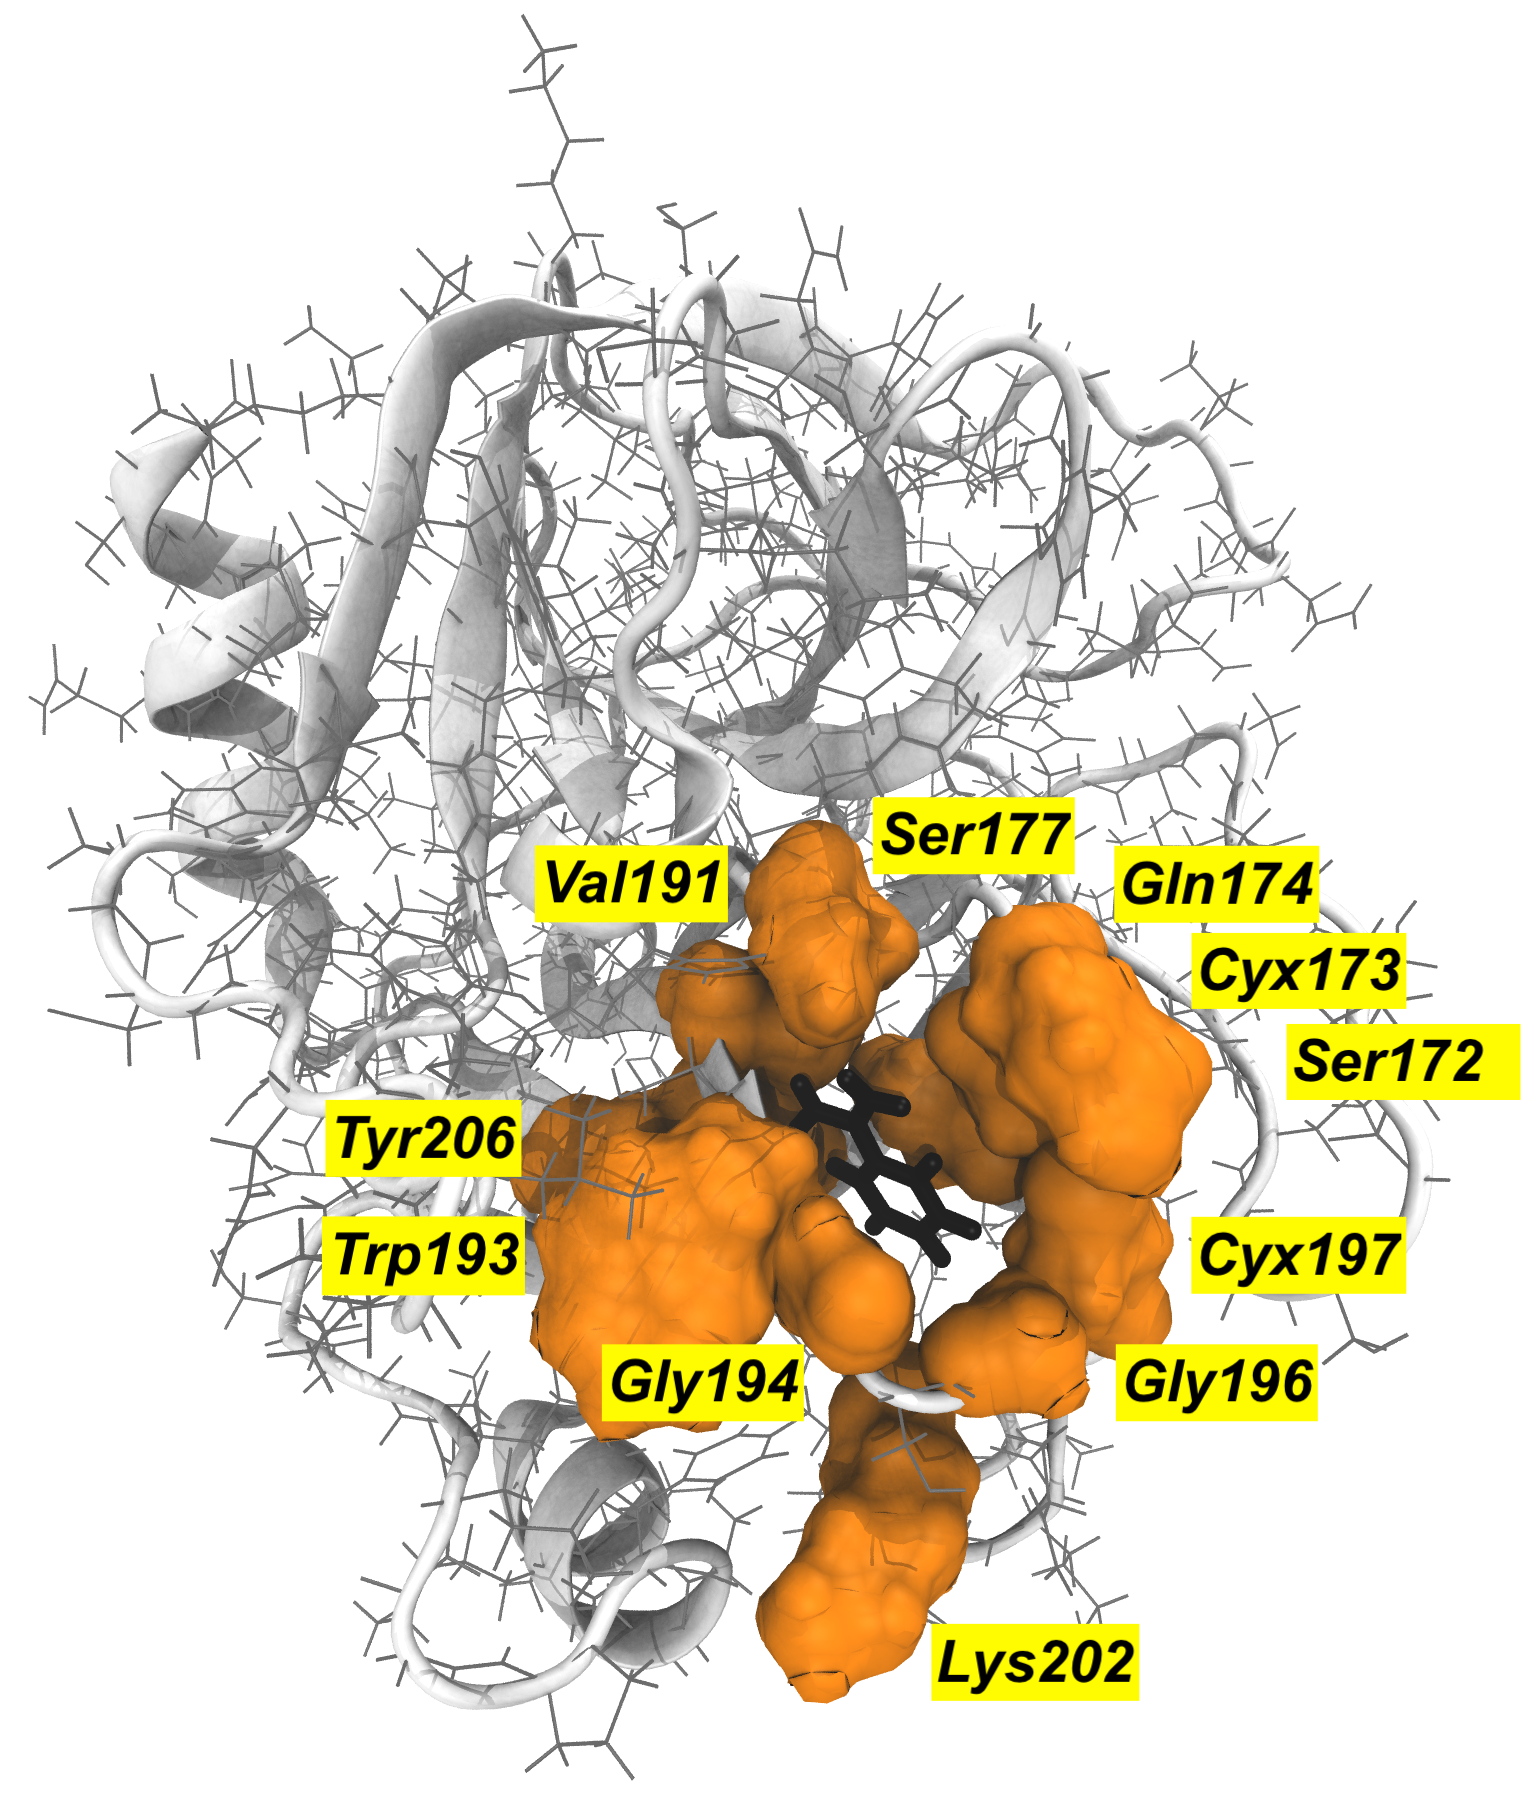
\includegraphics[scale=0.16]{images/figure7.png} 
\caption{Trypsin-benzamidine complex with the benzamidine molecule (in black) and surrounding residues constituting the binding site (in orange). The distance between the center of mass of the heavy atoms of the benzamidine molecule and the $\alpha$-carbons of the binding site residues constitute the collective variable.}
\label{figure7}
\end{figure} 

\noindent Now the model XML file and the SEEKR2 file tree have been generated in a separate \textit{SEEKR$\_$simulation} directory as specified explicitly by the <root$\_$directory> tag in the model input XML file, i.e., \textit{the input$\_$SMD$\_$HIDR.xml file}. HIDR will now employ SMD simulations to gradually pull the system into every anchor and save the structures for subsequent SEEKR2 calculations. To run SMD simulations with the HIDR algorithm, execute the following command in the terminal:

\begin{tcolorbox}[colback=black!8!white, colframe=black!50!black, fontlower=\tiny, left=2pt, right=2pt, top=2pt, bottom=2pt] 
\texttt{python $\sim$/seekrtools/seekrtools/hidr/hidr.py \textbackslash \linebreak any SEEKR$\_$simulation/model.xml -M SMD -p \textbackslash \linebreak trypsin$\_$benzamidine.pdb}
\end{tcolorbox}

\noindent This command is likely to run for hours or days, depending on the speed of the GPU. We can obtain a comprehensive overview of HIDR arguments by executing HIDR with the -h argument using the following python command:

\begin{tcolorbox}[colback=black!8!white, colframe=black!50!black, fontlower=\tiny, left=2pt, right=2pt, top=2pt, bottom=2pt] 
\texttt{python $\sim$/seekrtools/seekrtools/hidr/hidr.py -h}
\end{tcolorbox}

\noindent Several options in the HIDR program can be specified (described earlier in section  \ref{host_guest}), such as determining the equilibration steps before SMD simulations, allowing for some equilibration steps (settling steps) within each anchor after the SMD simulation has reached that particular anchor, and adjusting the speed of HIDR simulations. 

\noindent To keep the directory clean, we can optionally choose to delete the intermediate files:

\begin{tcolorbox}[colback=black!8!white, colframe=black!50!black, fontlower=\tiny, left=2pt, right=2pt, top=2pt, bottom=2pt] 
\texttt{rm trypsin$\_$benzamidine.inpcrd trypsin.pqr \textbackslash \linebreak trypsin$\_$benzamidine.pqr benzamidine.pqr}
\end{tcolorbox}

\subsection*{Stage 2: Run}
\vspace{2mm}

\noindent During the prepare stage of a SEEKR2 calculation, a file tree with essential files and directories is created at the location specified by the  <root$\_$directory> tag in the model input file. The run phase begins, executing SEEKR2  simulations based on the files and directories from the prepare stage. Within the main directory (\textit{SEEKR$\_$simulation}), a \textit{model.xml} file exists. The path to the \textit{model.xml} file is frequently used as an argument in many subsequent SEEKR2 processes, especially during the run phase. It is to be noted that directly altering the \textit{model.xml} without reinitiating \textit{prepare.py} is not recommended. The \textit{run.py} script initiates the run phase, and the following command launches the script to run MD simulations within the SEEKR2 milestones.

\begin{tcolorbox}[colback=black!8!white, colframe=black!50!black, fontlower=\tiny, left=2pt, right=2pt, top=2pt, bottom=2pt] 
\texttt{python $\sim$/seekr2/seekr2/run.py any \textbackslash \linebreak SEEKR$\_$simulation/model.xml}
\end{tcolorbox}

\noindent In the above command, "any" serves as the instruction argument for the \textit{run.py} script, prompting it to complete any pending MD or BD simulations. One might use "any$\_$md" or "any$\_$bd" to address unfinished MD or BD simulations. Please refer to the SEEKR2 documentation for a detailed set of available directives for the \textit{run.py} script.

\noindent Once we initiate the \textit{run.py} script, simulations will run until completion or interruption. The SEEKR2 framework saves checkpoints for both MD and BD simulations, allowing us to resume the calculation from where it was interrupted. To track the progress and convergence of the simulations, we  use the \textit{converge.py} script:

\begin{tcolorbox}[colback=black!8!white, colframe=black!50!black, fontlower=\tiny, left=2pt, right=2pt, top=2pt, bottom=2pt] 
\texttt{python $\sim$/seekr2/seekr2/converge.py any \textbackslash \linebreak SEEKR$\_$simulation/model.xml -l}
\end{tcolorbox}

\noindent Running the \textit{converge.py} script generates convergence plots, and images are saved in the \textit{plots$\_$and$\_$images} subfolder within the <root$\_$directory>. For additional arguments that can be used with both \textit{run.py} and \textit{converge.py}, we can run either script with the -h argument. 

\subsection*{Stage 3: Analyze}
\vspace{2mm}

\noindent The final stage within the SEEKR2 framework involves analyzing the results obtained from the simulations. This stage enables the construction of kinetics and thermodynamics profiles for the studied process. To execute the post-simulation SEEKR2 analysis:

\begin{tcolorbox}[colback=black!8!white, colframe=black!50!black, fontlower=\tiny, left=2pt, right=2pt, top=2pt, bottom=2pt] 
\texttt{python $\sim$/seekr2/seekr2/analyze.py \textbackslash \linebreak SEEKR$\_$simulation/model.xml}
\end{tcolorbox}

\begin{figure}[H]
\centering
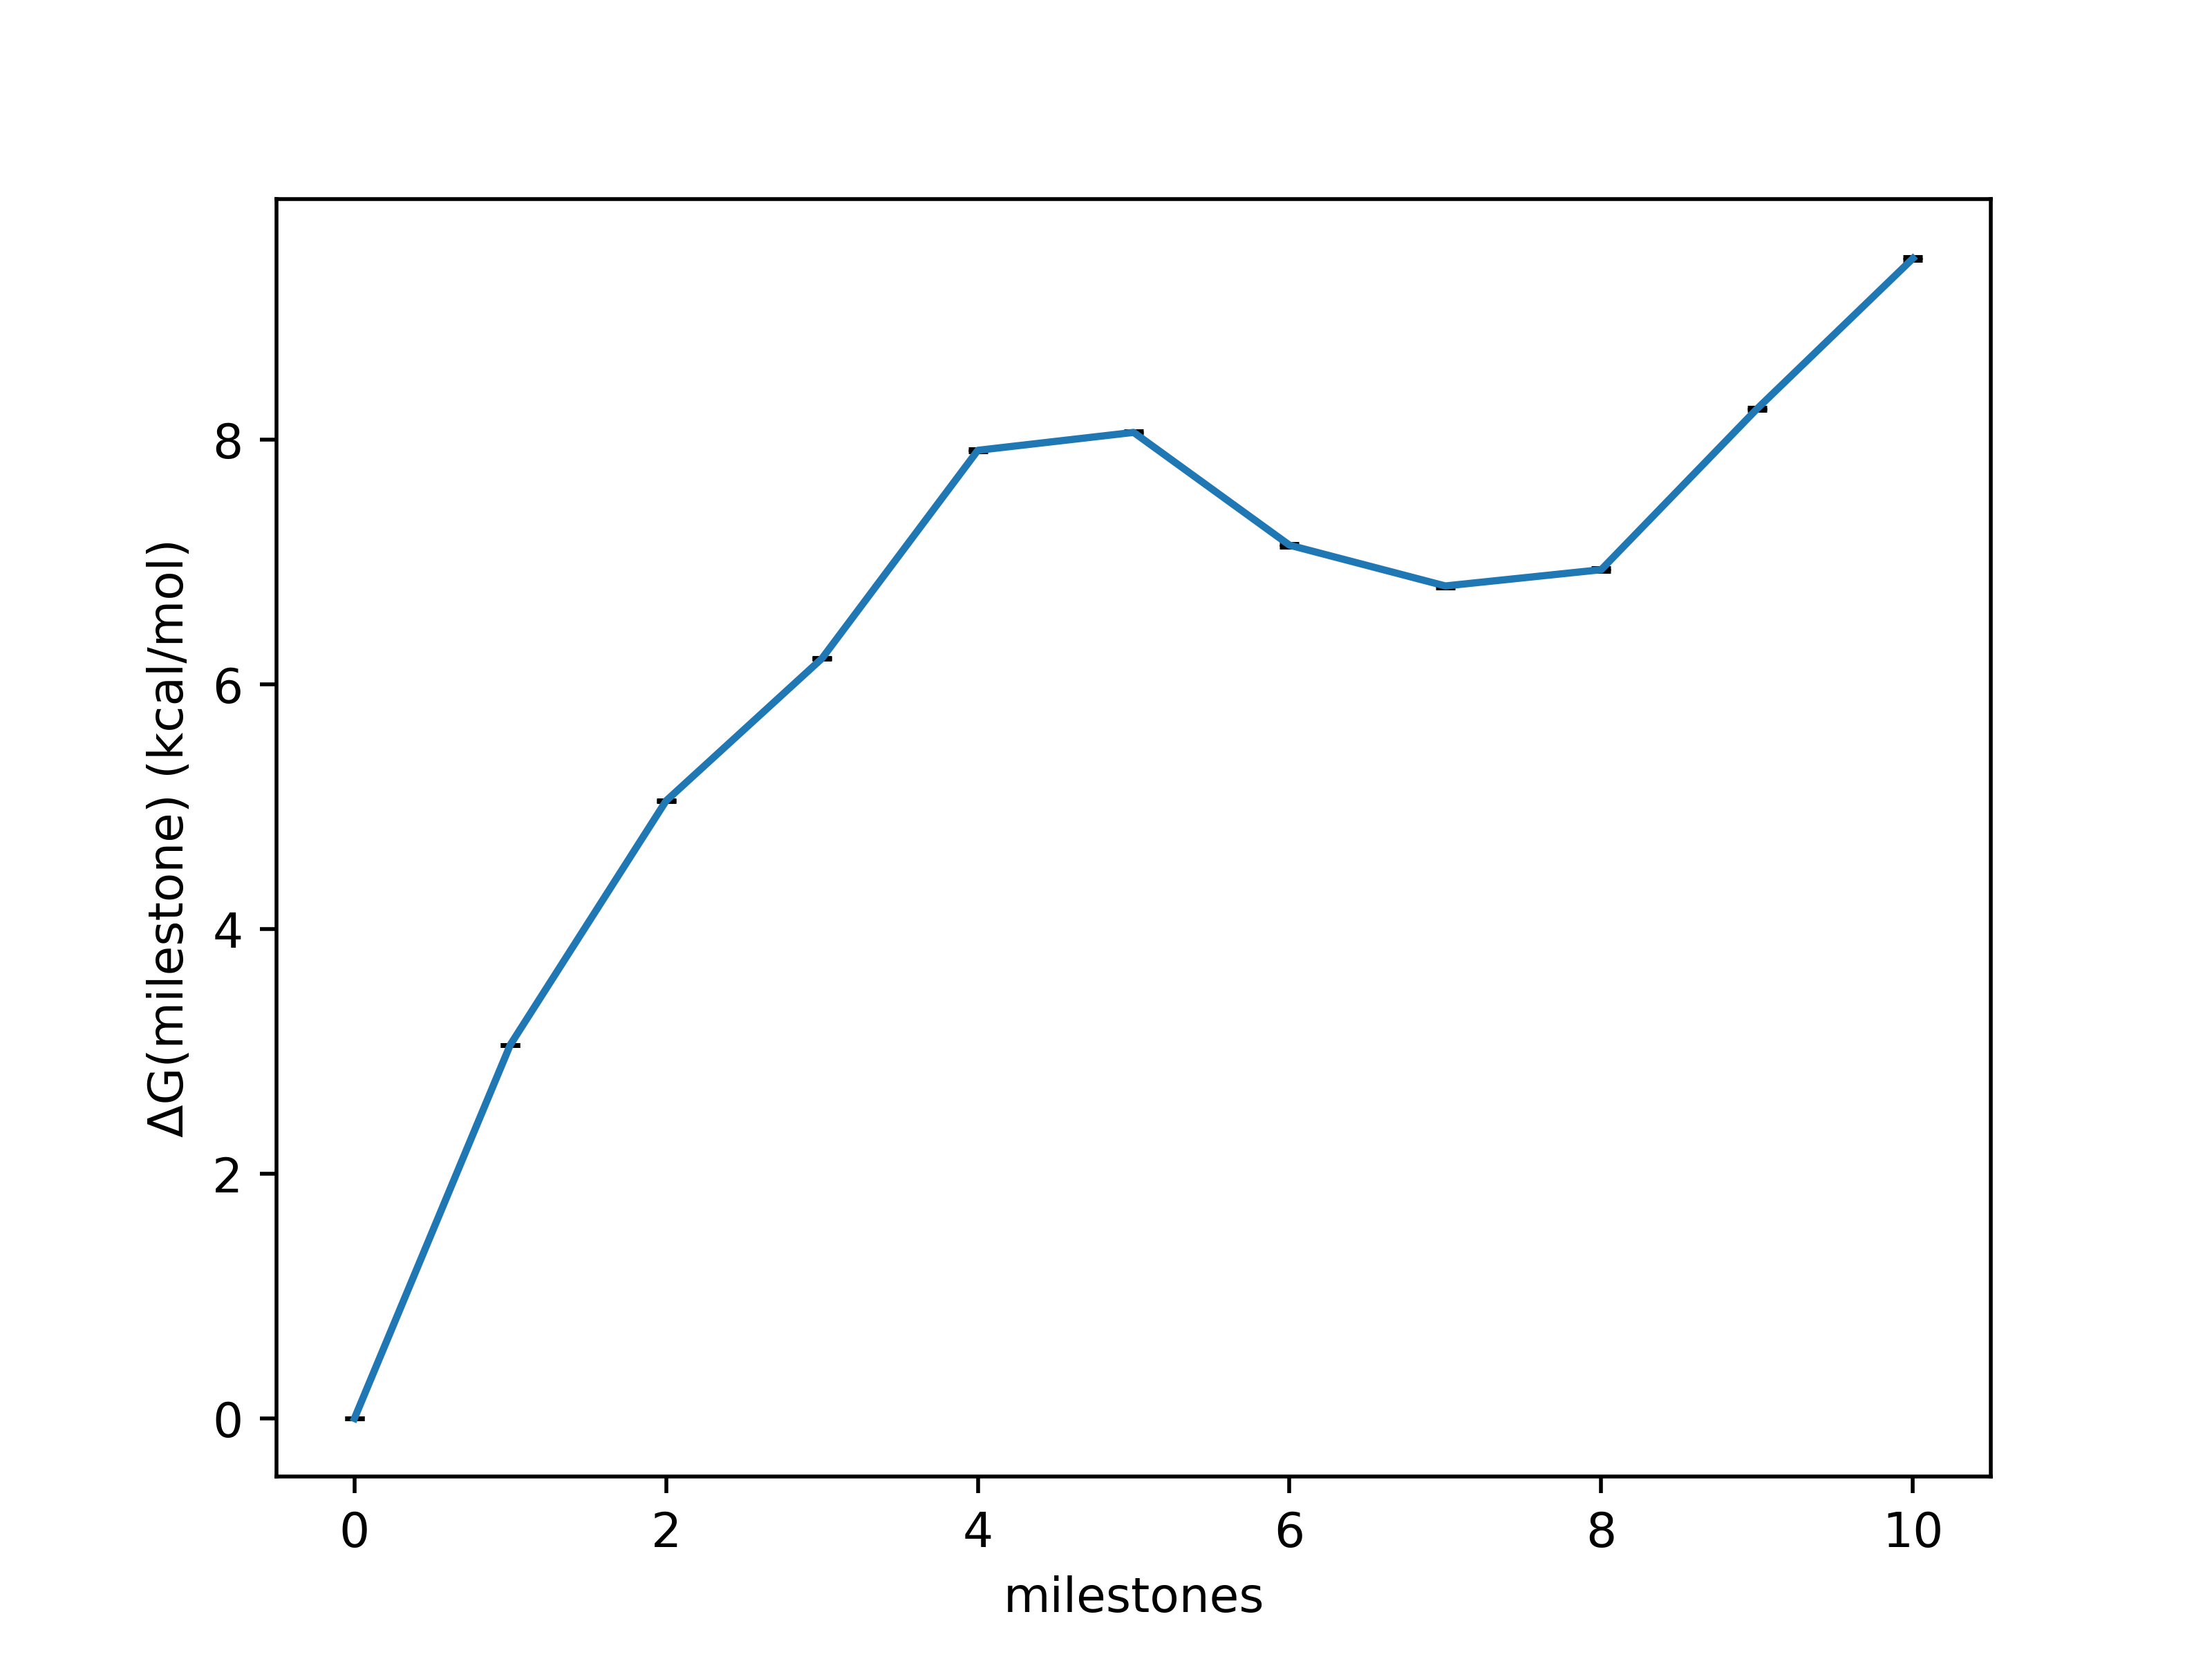
\includegraphics[scale=0.60]{images/figure8.png} 
\caption{Free energy profile per milestone ($\Delta$G\textsubscript{i}) obtained from the SEEKR2 milestoning method for the trypsin-benzamidine complex.}
\label{figure8}
\end{figure} 

\noindent The \textit{analyze.py} script takes the \textit{model.xml} file as an argument. It constructs the milestoning model, populates it with transition probabilities and simulation times within each milestone, and computes error margins. For a detailed understanding of the MMVT error margins, please refer to the SEEKR2 manuscript \cite{votapka2022seekr2}. Figure \ref{figure8} shows the free energy profile per milestone for the trypsin-benzamidine complex, obtained by executing the \textit{analyze.py} script.


\section{SEEKR2 benchmarking}
\vspace{2mm}


\noindent Benchmarking simulations were performed on a Linux machine with an NVIDIA Quadro RTX 5000 GPU with 16 GB RAM and an Intel Xeon W-10885M CPU. SEEKR2 milestoning simulations were run using the OpenMM version 7.7 for all the seven host-guest complexes and the trypsin benzamidine complexes, using 1 GPU with CUDA version 10.2. Table \ref{seekr_benchmarking} describes the benchmarking results. 

\begin{table}[H]
\centering
\begin{tabular}{ |p{5.2 cm}|p{2.0 cm}|}
\hline
\small{\textbf{Receptor-ligand complex}} & \small{\textbf{Benchmark (ns/day)}} \\
\hline
\small{BCD-1-butanol (5358 atoms)} & \small{569.60} \\
\hline
\small{BCD-1-napthylethanol (5362 atoms)}& \small{544.92} \\
\hline
\small{BCD-1-propanol (5361 atoms)} & \small{540.00} \\
\hline
\small{BCD-2-napthylethanol (5368 atoms)} & \small{526.27}  \\
\hline
\small{BCD-aspirin (5361 atoms)} & \small{559.68} \\
\hline
\small{BCD-methyl butyrate (5360 atoms)} & \small{556.87} \\
\hline
\small{BCD-terbutanol (5358 atoms)} & \small{564.95}  \\ 
\hline
\small{Trypsin-benzamidine (23036 atoms)} &  \small{171.11}  \\ 
\hline
\end{tabular}
\vspace{2mm}
\caption{Benchmarking rates for SEEKR2 simulations performed on the seven host-guest complexes and the trypsin-benzamidine complex performed on a single NVIDIA Quadro RTX 5000 GPU.}
\label{seekr_benchmarking}
\end{table}

\section{Conclusion}
\vspace{2mm}

SEEKR2 has emerged as a multiscale simulation tool designed to increase the speed and efficiency of calculating kinetic and thermodynamic properties of receptor-ligand binding and unbinding. This tutorial covers the underlying theory behind SEEKR2, describing how kinetic and thermodynamic properties are calculated. Beginning with the installation and setup, this manuscript guides the readers through the processes of preparing SEEKR2 simulations, highlighting essential options such as equilibration steps and adjusting the speed of HIDR simulations. The subsequent sections then provide a detailed walkthrough of the run and analysis stages, emphasizing the significance of files like \textit{model.xml} and scripts like \textit{run.py} and \textit{analyze.py}. Having achieved the learning outcomes outlined at the beginning, this tutorial is a comprehensive guide to installing and running SEEKR2 simulations, ensuring that even those unfamiliar with SEEKR2 can navigate its various features. We expect researchers are now well-positioned to apply SEEKR2 to their systems of interest.

\section*{Abbreviations}
\vspace{2mm}

\begin{tcolorbox}[colback=black!10!white, colframe=black!50!black, fontlower=\tiny, left=2pt, right=2pt, top=2pt, bottom=2pt]
\small{\textbf{SEEKR}: Simulation-enabled estimation of kinetic rates \\
\textbf{SEEKR2}: Simulation-enabled estimation of kinetic rates version 2 \\
\textbf{BD}: Brownian dynamics \\
\textbf{MD}: Molecular dynamics \\
\textbf{NAMD}: Nanoscale molecular dynamics \\
\textbf{VMD}: Visual molecular dynamics \\
\textbf{k\textsubscript{on}}: Association rate constant \\
\textbf{k\textsubscript{off}}: Dissociation rate constant \\
\textbf{CUDA}: Compute unified device architecture \\
\textbf{GPU}: Graphics processing unit \\
\textbf{CPU}: Central processing unit \\
\textbf{RCSB}: Research collaboratory for structural bioinformatics \\
\textbf{APBS}: Adaptive Poisson-Boltzmann solver \\
\textbf{MFPT}: Mean first-passage time \\
\textbf{MMVT}: Markovian milestoning with Voronoi tessellations \\
\textbf{PDB}: Protein data bank \\
\textbf{CV}: Collective variable \\
\textbf{COM}: Center of mass \\
\textbf{BSD}: Berkeley software distribution \\
\textbf{API}: Application programming interface \\
\textbf{SMD}: Steered molecular dynamics \\
\textbf{HIDR}: Holo insertion by directed restraints \\
\textbf{RAMD}: Random acceleration molecular dynamics \\
\textbf{HF-DFT}: Hartree-Fock with density functional theory \\
\textbf{GAMESS}: General atomic \& molecular electronic structure system \\
\textbf{MP2}: Møller-Plesset 2 \\
\textbf{AM1-BCC}: Austin model 1 with bond charge correction \\
\textbf{HMR}: Hydrogen mass repartitioning \\
\textbf{AMU}: Atomic mass unit \\
\textbf{frcmod}: Parameter modification file \\
\textbf{TIP3P}: Transferable intermolecular potential with 3 points \\
\textbf{TIP4Pew}: Transferable intermolecular potential with 4 points with Ewald techniques \\
\textbf{RAM}: Random-access memory \\
\textbf{RTX}: Real-time ray tracing }
\end{tcolorbox}

\section*{Author Contributions}
\vspace{2mm}
AA Ojha conceptualized and wrote the tutorial journal and is a developer of the SEEKR2 package. LW Votapka is the lead developer of the SEEKR2 package. GA Huber contributed to the Brownian dynamics section in the tutorial. RE Amaro provided support with computing resources. LW Votapka and RE Amaro provided guidance for tutorial development. S Gao extensively tested the SEEKR2 installation by following the tutorial and helped debug the instructions for installing, running, and analyzing SEEKR2 simulations. 

\section*{Other Contributions}
For a more detailed description of contributions from the community and others, see the GitHub issue tracking and changelog at \githubrepository.

\section*{Author Information}
\makeorcid

\section*{Potentially Conflicting Interests}
\vspace{2mm}
The authors declare no conflicting interests. 

\section*{Funding Information}
\vspace{2mm}
AA Ojha acknowledges the support of the Molecular Sciences Software Institute (MolSSI) fellowship under the National Science Foundation (NSF) grant OAC-1547580. GA Huber acknowledges support from National Institutes of Health (NIH) GM31749 and University of California San Diego. RE Amaro acknowledges support from NSF Extreme Science and Engineering Discovery Environment (XSEDE) CHE060063 and NIH GM132826.


\bibliography{ref}

\end{document}